%%
%%  Unified Adaptive-Friction + Navier-Stokes Paper
%%  Target: SIAM Journal on Applied Mathematics
%%
\documentclass[final]{siamltex}

%% ====================================================================
%%  Packages
%% ====================================================================
\usepackage{amsmath,amssymb,amsfonts}
\usepackage{mathtools}
\usepackage{bm}
\usepackage{booktabs}
\usepackage{algorithm}
\usepackage{algorithmic}
\usepackage{graphicx}
\usepackage{hyperref}
\usepackage{url}
\usepackage{microtype}
\usepackage{xcolor}
\usepackage{appendix}
\usepackage{multirow}

%% ====================================================================
%%  Notation & shortcuts
%% ====================================================================
\newcommand{\R}{\mathbb{R}}
\newcommand{\E}{\mathbb{E}}
\newcommand{\N}{\mathbb{N}}
\newcommand{\T}{\mathbb{T}}
\newcommand{\norm}[1]{\lVert #1 \rVert}
\newcommand{\inner}[2]{\langle #1,\, #2 \rangle}
\providecommand{\grad}{\nabla}
\newcommand{\Ebs}{E_{\mathrm{BS}}}
\newcommand{\Cman}{\mathcal{C}^*}
\newcommand{\Xst}{X^*}
\newcommand{\Lpair}{L_{\mathrm{pair}}}
\newcommand{\lmin}{\lambda_{\min}}
\newcommand{\lmax}{\lambda_{\max}}
\newcommand{\costheta}{\cos\theta}
\newcommand{\ddt}{\tfrac{d}{dt}}
\DeclareMathOperator{\erf}{erf}
\DeclareMathOperator{\sym}{sym}
\DeclareMathOperator{\ind}{ind}
\DeclareMathOperator{\tr}{tr}

%% ====================================================================
%%  Extra theorem-like environments (SIAM provides theorem, lemma,
%%  corollary, proposition, definition)
%% ====================================================================
\newtheorem{assumption}[theorem]{Assumption}
\newtheorem{remark}[theorem]{Remark}

%% ====================================================================
%%  Title & metadata
%% ====================================================================
\title{Systemic Risk as Geometry: Blind-Spot Decomposition, Adaptive
Friction, and Applications to Finance, Energy, and Navier--Stokes
Regularity\thanks{Submitted to the editors \today.}}

\author{Odeyemi Olusegun\thanks{Independent Researcher, London, UK.
(\texttt{segettii@gmail.com}).
ORCID: 0009-0004-2309-6436.}}

\begin{document}
\maketitle

\pagestyle{myheadings}
\thispagestyle{plain}
\markboth{O.\ ODEYEMI}{SYSTEMIC RISK AS GEOMETRY}

%% ====================================================================
%%  Abstract
%% ====================================================================
\begin{abstract}
We propose a geometric framework for detecting and controlling
structural instability in coupled dynamical systems by recasting
the problem in terms of energy-topology equivalence.
$N$ interacting agents evolve under a
potential $\Phi$ whose pairwise term encodes contagion; a
\emph{Blind-Spot Decomposition Theory} (BSDT) energy functional
$\Ebs$, calibrated on normal-period data, is shown to be
topologically equivalent to $\Phi$ via a \emph{Morse-index
equivalence} (Theorem~C:
$\mathrm{ind}_{\Ebs}(X_c) = \mathrm{ind}_\Phi(X_c)$ at every
critical point, with two-sided gradient bounds
$c_1\norm{\grad\Phi}\le\norm{\grad\Ebs}\le c_2\norm{\grad\Phi}$
and homotopy equivalence of sublevel sets).
This equivalence recasts the instability detection problem as a
control problem: a \emph{critical manifold} $\Cman$, characterised
by the Morse-index jump $\mathrm{ind}=0\to\mathrm{ind}\ge 1$,
separates a stable from an unstable regime.  Adaptive friction
$\gamma^*(X)=\alpha/\lmax(D^2\Phi_{\mathrm{pair}})$ achieves
marginal stability where every fixed coupling fails
(Theorem~\ref{thm:phase})---a formal characterisation of
procyclicality in financial regulation.

Two physics-based \emph{System Mode engines} operationalise the
theory: a Lennard-Jones 6--12 \emph{Molecular Engine} and a
Gaussian-attraction / Coulomb-repulsion \emph{Gravity Mode Engine},
unified through a common Lyapunov~v2 stabiliser with Armijo
backtracking ($c=10^{-4}$), Input-to-State Stability (ISS) margins,
and La~Salle convergence certification ($\tau_{\mathrm{LS}}=10^{-5}$,
patience~5).  Both engines share a \emph{Fused Topological Scoring}
architecture: Morse critical-point alarm, Betti barcode persistence,
and a four-operator UDL stack (Phase, Topological, KernelRKHS, Rank)
fused at equal weight after min-max normalisation.  The BSDT
channel weights are determined by a closed-form Fisher
variance-ratio statistic (zero label leakage).  A
\emph{SpectraFalseAlarmFilter} gates scores by topological
persistence, and a \emph{FARTargetCalibrator} enforces a target
false-alarm rate via piecewise-linear rescaling.

A \emph{Universal Conformal Scoring} layer provides
distribution-free anomaly detection: each engine's physics
simulation produces raw scores that are calibrated via split
conformal prediction, yielding valid $p$-values under exchangeability
alone.  Panel-level aggregation (rolling mean, P90, max, standard
deviation, momentum) fuses point-level scores into quarter-level
summaries; rank-normalised fusion selects the better of point-level
and panel-level views per dataset automatically.  On the ERCOT
benchmark the Hybrid Engine achieves AUC~$=0.9997$; on the G-SIB
bank-level panel, quarter-level conformal fusion lifts the Gravity
Engine from $0.766$ to $0.806$ ($+4.0$\,pp) while preserving zero
COVID false alarms.
All reported lead times are measured under a strictly causal
expanding-window protocol: each score at quarter $t$ uses only
information available up to $t$, with no future observations,
no future labels, and no hindsight re-estimation.

The extended framework is validated on FDIC banking data (6-quarter
GFC lead, AUROC~$= 0.867$ with adaptive calibration, zero false
alarms at 38.5\% recall and 100\% precision), the Terra/Luna
collapse ($r=0.996$, $+30$\,h lead), the Texas ERCOT grid
($+72$\,h lead), and three new sensitive-sector benchmarks: FRED
macroeconomic indicators (AUC $= 0.9999$), ERCOT energy-grid
dispatch (AUC $= 0.9940$), and a prospective G-SIB bank-level
panel where Mol+ExpoGate first alarms at 2007-Q4---two quarters
before the Bear~Stearns collapse.
The BSDT channels transfer to three-dimensional incompressible
Navier--Stokes, where adaptive viscosity maintains the
production/dissipation ratio at $0.500\pm 0.005$ across Reynolds
numbers $314$--$6283$.
\end{abstract}

\begin{keywords}
systemic risk, Lyapunov stability, entropy production, Onsager
gradient flow, phase transition, adaptive friction,
Navier--Stokes regularity, enstrophy, blind-spot decomposition,
online convex optimisation, physics-based scoring,
Lennard-Jones potential, fused topology,
false-alarm-rate calibration
\end{keywords}

\begin{AMS}
91G45, 37N40, 35Q30, 76D03, 93D20, 91B55
\end{AMS}

%% ====================================================================
%%  1.  INTRODUCTION
%% ====================================================================
\section{Introduction}\label{sec:intro}

The 2008 Global Financial Crisis demonstrated that systemic risk
resides not in individual institutions but in the geometry of
their interactions. Existing frameworks---CoVaR
\cite{adrian2016covar}, SRISK \cite{brownlees2017srisk},
network contagion models \cite{acemoglu2015systemic,
elliott2014financial}---detect stress \emph{after} it
propagates. This paper proposes a geometric framework for
detecting and characterising structural instability in coupled
systems, and derives adaptive stabilisation as a direct consequence
of the underlying energy-topology structure.  The key insight is
that a detection functional calibrated on normal-period data
shares the same Morse-index landscape as the interaction
energy---so detecting instability and controlling it become two
views of the same geometric object.

Formally, an \emph{equivalence theorem} links two seemingly
unrelated objects: (i)~a \emph{detection} functional $\Ebs$
measuring deviation from historical normality, and (ii)~the
\emph{interaction energy} $\Phi$ governing agent dynamics.
Theorem~C establishes that $\Ebs$ and $\Phi$ share the same
Morse-index structure at every critical point, that their sublevel
sets are homotopy equivalent, and that gradient norms are equivalent
up to computable constants.  This identification transforms
the instability detection problem into a control problem: damping
the system using $\grad\Ebs$ stabilises it because $\grad\Ebs$ and
$\grad\Phi$ are geometrically aligned.  The Morse-index jump from
$0$ to $\ge 1$ provides a topological instability signal that is
structurally invariant under perturbation and decoupled from the
Lyapunov descent certificate used to guarantee iteration
convergence.

A \emph{critical manifold} $\Cman$ separates two dynamical
regimes. Below $\Cman$, any fixed coupling suffices for stability.
Above $\Cman$, no constant friction stabilises all configurations
(Theorem~\ref{thm:phase}). The system requires \emph{adaptive}
friction $\gamma^*(X)$ that tracks the spectral radius of the
pairwise Hessian in real time. This phase-transition structure
provides a rigorous dynamical-systems characterisation of
procyclicality: time-invariant regulatory rules (such as Basel
III's fixed countercyclical capital buffer) fail
\emph{structurally}, not merely in practice.

\paragraph{Contributions.}
This paper makes nine contributions:
\begin{enumerate}
\item \textbf{Blind-Spot Decomposition Theory (BSDT).} Four
  deviation operators ($\delta_C$: camouflage, $\delta_G$: feature
  gap, $\delta_A$: activity anomaly, $\delta_T$: temporal novelty)
  define $\Ebs$, a composite energy functional that decomposes
  structural instability into geometrically interpretable channels,
  calibrated entirely on normal-period data.

\item \textbf{Equivalence Theorem (Theorem~C) and Entropy Structure
  (Theorem~\ref{thm:entropy}).} Morse-index equivalence
  $\mathrm{ind}_{\Ebs}=\mathrm{ind}_\Phi$ at every critical point,
  topological energy equivalence via homotopy of sublevel sets,
  two-sided gradient bounds, and decoupled stabilisation establish
  $\Ebs$ as a Lyapunov function for the potential flow
  (Proposition~\ref{prop:separation}); the system is a generalised
  Onsager gradient flow with non-negative entropy production
  $\sigma(X) = \gamma(\Ebs)\norm{\grad\Ebs}^2 \ge 0$.
  This equivalence provides the mathematical basis for both
  detecting instability (via the Morse-index jump) and controlling
  it (via gradient-aligned damping).

\item \textbf{Critical manifold and phase transition
  (Theorem~\ref{thm:phase}).} A spectral threshold determines
  where constant friction fails and adaptive friction succeeds,
  providing a rigorous dynamical-systems characterisation of why
  constant-parameter regulation fails in complex networks.

\item \textbf{System Mode engines
  (Section~\ref{sec:engines}).}  A Lennard-Jones Molecular Engine
  and a Gaussian/Coulomb Gravity Mode Engine share an identical
  post-simulation operator stack (Phase, Topological, KernelRKHS,
  Rank) fused via a Morse/Betti/UDL scoring architecture.
  A Hybrid Engine selects the optimal convex blend by
  cross-validated AUROC maximisation.

\item \textbf{Lyapunov v2 convergence guarantee
  (Proposition~\ref{prop:lyapv2}).}  Three-part certificate:
  Armijo--ISS descent, La~Salle invariance, and coercivity ensure
  convergence for all engines with $O(nk)$ per-step complexity.

\item \textbf{Online algorithm with $O(\sqrt{T})$ regret.} The
  adaptive coupling is implementable via online gradient descent
  with power-iteration spectral estimates.

\item \textbf{Empirical validation.} On FDIC banking data
  ($T=140$ quarters, $N=7$ institution types, $d=6$ features), the
  framework achieves a 6-quarter GFC early warning, AUROC $\ge
  0.70$.  On FRED macroeconomic data, AUC $= 0.9999$; on ERCOT
  energy-grid dispatch, AUC $= 0.9940$; on a prospective G-SIB
  bank-level panel, $z > 2$ six quarters before Lehman.

\item \textbf{Universal conformal scoring
  (Section~\ref{sec:conformal}).}  Split conformal prediction
  calibrates each engine's raw physics scores into valid
  $p$-values under exchangeability alone.  Panel-level
  aggregation and rank-normalised fusion automatically select
  the better of point-level and quarter-level scoring per
  dataset, improving Gravity AUC on the G-SIB panel by
  $+4.0$\,pp with no additional hyperparameters.

\item \textbf{Cross-domain universality.} The same geometric
  framework, without re-training, characterises structural
  instability in the Terra/Luna collapse ($r=0.996$),
  the Texas ERCOT grid failure ($+72$\,h lead), and
  Navier--Stokes turbulence---suggesting that the energy-topology
  structure is a general feature of coupled dynamical systems,
  not specific to any single domain.

\item \textbf{Extension to Navier--Stokes.} The BSDT channel
  structure transfers to three-dimensional incompressible
  Navier--Stokes, where adaptive viscosity suppresses enstrophy
  growth and maintains bounded production/dissipation ratios---a
  pathway toward regularity results.
\end{enumerate}

\paragraph{Related work.}
Network-based systemic risk models
\cite{acemoglu2015systemic,elliott2014financial} capture topology
but not dynamics. Market-based measures (CoVaR, SRISK) require
market prices and operate at the market frequency, missing
slow-moving structural drift on regulatory balance sheets.
The May--Levin--Sugihara programme \cite{may2008complex} imports
ecological stability analysis but lacks operational control
algorithms. Our framework complements these by providing feedback
control with formal stability guarantees. For the Navier--Stokes
connection, the Beale--Kato--Majda criterion \cite{bkm1984} and
Ladyzhenskaya's classical estimates \cite{lady1969} provide the
regularity backdrop.

\paragraph{Outline.}
Section~\ref{sec:model} introduces the agent model and BSDT.
Section~\ref{sec:equiv} proves Theorem~C. Section~\ref{sec:damping}
establishes the phase transition. Section~\ref{sec:online} presents
the online algorithm and optimal policy.
Section~\ref{sec:engines} introduces the System Mode engines
(Molecular, Gravity, Hybrid) and their shared fused scoring
architecture. Section~\ref{sec:empirical}
validates on financial data. Section~\ref{sec:crossdomain} extends
to crypto and energy systems. Section~\ref{sec:ns} transfers the
framework to Navier--Stokes. Section~\ref{sec:discussion}
concludes.


%% ====================================================================
%%  2.  AGENT MODEL AND BSDT
%% ====================================================================
\section{Mathematical Framework}\label{sec:model}

\subsection{Agent Model and GravityEngine Dynamics}\label{sec:agents}

Consider $N$ interacting institutions, each described by a state
vector $x_i(t)\in\R^d$ of financial characteristics. The joint
state $X(t)=(x_1,\ldots,x_N)\in\R^{N\times d}$ evolves under the
gradient flow
\begin{equation}\label{eq:gradflow}
  \dot{X} = F(X) = -\grad\Phi(X),
\end{equation}
where $\Phi:\R^{N\times d}\to\R$ decomposes as
\begin{equation}\label{eq:potential}
  \Phi(X) = \underbrace{\frac{\alpha}{2}\sum_{i=1}^{N}
  \norm{x_i-\mu}^2}_{\text{radial spring (mean-reversion)}}
  + \underbrace{\sum_{i<j}\phi(\norm{x_i-x_j})}_{\text{pairwise
  interaction}}.
\end{equation}
The pairwise potential $\phi(r)=\gamma\frac{\sigma\sqrt{\pi}}{2}
\erf(r/\sigma)-\gamma\lambda\log(r+\varepsilon)$ combines
short-range Gaussian attraction with long-range logarithmic
repulsion, giving clustering at equilibrium distance $r^*=
\sigma\sqrt{\log(1/\lambda)}$.

The \emph{unique Nash equilibrium} under the friction game
$\min_{\ell_i}[\text{private cost}_i+\gamma\cdot
\text{systemic externality}_i]$ is $\ell_i^*(\gamma)=
(\alpha+\gamma w_i)^{-1}r_i$, where $w_i$ is institution~$i$'s
network centrality and $r_i$ its return on assets.
The optimal coupling $\gamma^*$ internalises the Pigouvian
externality $\tau_i^*=\gamma^*\,\partial E/\partial\ell_i$,
proportional to each institution's marginal contribution to system
energy.

\subsection{Blind-Spot Decomposition Theory (BSDT)}\label{sec:bsdt}

BSDT decomposes systemic risk into four geometrically orthogonal
channels of deviation from the normal-period distribution
$\mathcal{N}$:
\begin{enumerate}
\item \textbf{Camouflage} ($\delta_C$): Mahalanobis distance from
  $\mathcal{N}$. Detects states that appear individually normal but
  are collectively anomalous:
  $\delta_C(X) = [(X{-}\mu_0)^\top\Sigma_0^{-1}(X{-}\mu_0)]^{1/2}$.

\item \textbf{Feature Gap} ($\delta_G$): PCA residual in
  low-variance directions. Detects motion into historically
  unoccupied subspaces: $\delta_G(X)=\norm{(I-P_k)X}$.

\item \textbf{Activity Anomaly} ($\delta_A$): Excess velocity
  relative to normal-period dynamics:
  $\delta_A=\max(0,\norm{\dot{x}_i}-v_0)$.

\item \textbf{Temporal Novelty} ($\delta_T$): Negative log-density
  under a KDE of historical states:
  $\delta_T=-\log\hat{p}(x_i(t))$.
\end{enumerate}

The \emph{blind-spot energy functional} is the weighted composite
\begin{equation}\label{eq:ebs}
  \Ebs(X) = \sum_{k=1}^{4}w_k\,\psi_k(\delta_k(X))
  + \sum_{i<j}\phi(\norm{x_i-x_j}),
\end{equation}
where $\psi_k:\R^+\to\R^+$ are convex, non-decreasing,
1-Lipschitz link functions with $\psi_k(0)=0$. The pairwise
potential in $\Ebs$ coincides with $\Phi_{\mathrm{pair}}$,
ensuring structural compatibility between detection and dynamics.

\paragraph{Fisher Variance-Ratio Weighting.}
The channel weights $w_k$ are determined entirely from the data,
requiring no labelled examples.  Let $m_k = |\delta_k(X)|$ be the
channel magnitude vector across all $n$ observations.  We split the
data at the 80th and 50th percentiles of total magnitude
$M = \sum_k m_k$ into ``high'' and ``low'' groups and compute the
\emph{Fisher variance ratio}:
\begin{equation}\label{eq:fisher_vr}
  \mathrm{FR}_k
  = \frac{(\mu_k^{\mathrm{high}} - \mu_k^{\mathrm{low}})^2}
         {\mathrm{Var}_k^{\mathrm{high}}
          + \mathrm{Var}_k^{\mathrm{low}}},
  \qquad
  w_k = \frac{\mathrm{FR}_k}{\sum_{j}\mathrm{FR}_j}.
\end{equation}
This closed-form weighting adaptively assigns importance to
whichever channels best separate high-deviation from low-deviation
regimes, with zero label leakage by construction.

\paragraph{Sign Discovery and Herding.}
The sign $\mathrm{sgn}(\mu_k^{\mathrm{high}}-\mu_k^{\mathrm{low}})$
reveals the \emph{direction} of each channel's deviation during
stress.  On financial data, $\delta_C$ receives a \emph{negative}
Fisher coefficient---curvature \emph{collapses} during crises,
the fingerprint of herding: agents crowd into identical positions,
reducing the loss-landscape curvature to near zero.  Meanwhile
$\delta_T$ (temporal novelty) receives the strongest positive
weight, indicating that crises produce genuinely unprecedented
states.

The \emph{Multi-Factor Latent Score} (MFLS) is the Frobenius norm
$\norm{\grad\Ebs(X_t)}_F$, serving as a scalar early-warning
signal.


%% ====================================================================
%%  3.  THE EQUIVALENCE THEOREM
%% ====================================================================
\section{The Equivalence Theorem}\label{sec:equiv}

We work with a fixed reference measure $\mathcal{N}$ (the
normal-period distribution) and assume $\Phi$ satisfies
Assumptions~\ref{ass:reg}--\ref{ass:sep} below.

\subsection{Assumptions}

\begin{assumption}[Regularity]\label{ass:reg}
$\Phi\in C^2(\R^{N\times d})$ is coercive: $\Phi(X)\to+\infty$ as
$\norm{X}\to\infty$. Every sublevel set $\mathcal{L}_c:=
\{X:\Phi(X)\le c\}$ is compact, with Lipschitz constant $L_c$ for
$\grad\Phi$ on $\mathcal{L}_c$.
\end{assumption}

\begin{assumption}[Strict local minimum]\label{ass:equil}
The equilibrium $\Xst$ satisfies $\grad\Phi(\Xst)=0$ and
$H^*:=D^2\Phi(\Xst)\succ 0$.
\end{assumption}

\begin{assumption}[BSDT regularity]\label{ass:bsdt}
Each $\delta_i:$ $\R^{N\times d}\to\R^+$ is $C^1$ and
$K_i$-Lipschitz on $\mathcal{L}_c$. Each $\psi_i:\R^+\to\R^+$ is
convex, non-decreasing, 1-Lipschitz, with $\psi_i(0)=0$.
\end{assumption}

\begin{assumption}[Separation]\label{ass:sep}
\begin{enumerate}
\item[\textup{(S1)}] \textbf{Non-degeneracy.}
  There exists $\nu>0$ such that for every $X\in\mathcal{L}_c$
  with $\grad\Phi(X)\neq 0$, at least one index
  $i=i(X)\in\{1,\ldots,4\}$ satisfies
  $\norm{\grad_X\delta_i(X)}\ge\nu\norm{\grad\Phi(X)}$.
\item[\textup{(S2)}] \textbf{Monotonicity.}
  For all $i$ and all $X\in\mathcal{L}_c$:
  $\inner{\grad_X\delta_i(X)}{\grad\Phi(X)}\ge 0$.
\end{enumerate}
\end{assumption}

\begin{assumption}[Morse non-degeneracy]\label{ass:morse}
At every critical point $X_c$ of $\Ebs$ (i.e.\ $\grad\Ebs(X_c)=0$),
the Hessian $D^2\Ebs(X_c)$ is non-degenerate:
$\det(D^2\Ebs(X_c))\neq 0$.  Likewise, at every critical point
$X_c$ of $\Phi$, $\det(D^2\Phi(X_c))\neq 0$.
\end{assumption}

\begin{remark}\label{rem:morse_generic}
Morse non-degeneracy is a generic condition: the set of potentials
violating it has infinite codimension in the $C^2$ topology.  For
the LJ~6--12 and Gaussian/Coulomb potentials
(\eqref{eq:lj}, \eqref{eq:gravforce}), non-degeneracy holds at
all finite-energy critical points by direct computation of the
Hessian eigenvalues.
\end{remark}

\begin{remark}\label{rem:monotonicity}
Part~(S2) holds naturally: each $\delta_i$ measures deviation from
normal-period behaviour, so $\delta_i$ increases along directions
of increasing instability $\Phi$.  For the Mahalanobis channel
$\delta_C$, the gradient $\Sigma_0^{-1}(X{-}\mu_0)/\delta_C$
shares the outward radial direction with $\grad\Phi$.  For
$\delta_G$, the orthogonal projector $(I{-}P_k)$ either gives zero
or increases in directions exiting the principal subspace.
Part~(S1) is the existential (rather than universal) requirement
that the \emph{composite} detection gradient is not degenerate.
\end{remark}

\begin{proposition}[Structural derivation of the separation
condition]\label{prop:separation}
Let $\Sigma_0\succ 0$ be the Ledoit--Wolf shrinkage estimator
with condition number $\kappa(\Sigma_0)$. Then:
\begin{enumerate}
\item[\textup{(i)}] $\delta_C$ satisfies~(S1) with $\nu_C=
  \kappa(\Sigma_0)^{-1}[\alpha\sqrt{\lmax(\Sigma_0)}]^{-1}$,
  determined entirely by spectral properties of $\Sigma_0$ and the
  spring constant~$\alpha$. Monotonicity~(S2) holds because
  $\inner{\grad\delta_C}{\grad\Phi}\ge 0$ in a neighbourhood
  of~$\Xst$ (the Mahalanobis and potential gradients share the
  outward radial direction).

\item[\textup{(ii)}] $\delta_G$ satisfies $\norm{\grad_X\delta_G}=1$
  whenever $\delta_G>0$, giving unconditional~(S1). At points
  with $\delta_G=0$, the feature gap vanishes and cannot be the
  active channel; another $\delta_i$ provides the bound.

\item[\textup{(iii)}] $\delta_A$ satisfies~(S1)
  with $\nu_A=2\eta(\lambda_u-\alpha)/L_c$ in the super-critical
  region.

\item[\textup{(iv)}] $\delta_T$ satisfies~(S1)
  with $\nu_T=h^{-1}/L_c$ outside the kernel bandwidth~$h$.
\end{enumerate}
Since each channel individually satisfies~(S1) in a region,
and the regions cover $\mathcal{L}_c$, the composite $\Ebs$
inherits the existential bound with
$\nu\ge\max(\nu_C,\nu_G,\nu_A,\nu_T)$ at each~$X$.
\end{proposition}

\begin{proof}
Part~(i): $\grad_X\delta_C=\Sigma_0^{-1}(X{-}\mu_0)/\delta_C(X)$;
by the Rayleigh quotient,
$\norm{\Sigma_0^{-1}v}^2\ge\lmax(\Sigma_0)^{-2}\norm{v}^2$, and
$\delta_C(X)\le\sqrt{\lmax(\Sigma_0)}\norm{v}$. Combining with
$\norm{\grad\Phi(X)}\le L_c\norm{X{-}\Xst}$ near $\Xst$ gives the
bound. Part~(ii): $(I{-}P_k)$ is an orthogonal projector, so
$\grad_X\norm{(I{-}P_k)X}$ is a unit vector. Parts~(iii)--(iv)
follow from direct gradient computation using super-critical
growth estimates (Theorem~\ref{thm:phase}) and score-function
lower bounds.
\end{proof}

\subsection{Gradient Alignment}\label{sec:gradient}

\begin{lemma}[Gradient of $\Ebs$]\label{lem:grad_ebs}
Under Assumption~\ref{ass:bsdt}, $\Ebs$ is $C^1$ with
\[
  \grad\Ebs(X) =
  \underbrace{\textstyle\sum_{i=1}^{4}\psi_i'(\delta_i)\grad_X\delta_i}_
  {\grad\Ebs^{\mathrm{dev}}}
  + \underbrace{\grad_X\textstyle\sum_{i<j}
  \phi(\norm{x_i{-}x_j})}_{\grad\Ebs^{\mathrm{pair}}
  =-F_{\mathrm{pair}}}.
\]
\end{lemma}

\begin{lemma}[Upper bound]\label{lem:upper}
Under Assumptions~\ref{ass:reg}--\ref{ass:bsdt}, on
$\mathcal{L}_c$ there exists $c_2>0$ such that
$\norm{\grad\Ebs(X)}\le c_2\norm{\grad\Phi(X)}$.
\end{lemma}

\begin{lemma}[Lower bound]\label{lem:lower}
Under Assumptions~\ref{ass:reg}--\ref{ass:sep}, on
$\mathcal{L}_c$ there exists $c_1>0$ such that
$\norm{\grad\Ebs(X)}\ge c_1\norm{\grad\Phi(X)}$.
\end{lemma}

Proofs of the upper and lower bounds follow from the triangle
inequality, the Lipschitz properties of $\delta_i$, and the
separation condition. Full details are in
Appendix~\ref{app:proofs}.

\subsection{Theorem~C: Full Statement and Proof}\label{sec:thmC}

\begin{theorem}[Equivalence of Blind-Spot Geometry and Instability
Energy]\label{thm:equiv}
Let Assumptions~\ref{ass:reg}--\ref{ass:morse} hold and let $\Xst$
be a strict local minimum of $\Phi$. Then on any sublevel set
$\mathcal{L}_c$:

\begin{enumerate}
\item[\textup{(C1)}] \textbf{Morse-index equivalence.}
  At every critical point $X_c\in\mathcal{L}_c$
  (where $\grad\Phi(X_c)=0$ and $\grad\Ebs(X_c)=0$),
  \begin{equation}\label{eq:morse_index}
    \mathrm{ind}_{\Ebs}(X_c) = \mathrm{ind}_{\Phi}(X_c),
  \end{equation}
  where $\mathrm{ind}_f(X_c)$ denotes the \emph{Morse index}
  (number of negative eigenvalues of $D^2 f(X_c)$).

\item[\textup{(C2)}] \textbf{Topological energy equivalence.}
  The sublevel sets $\mathcal{L}_c^{\Ebs}:=\{X:\Ebs(X)\le c\}$
  and $\mathcal{L}_c^{\Phi}:=\{X:\Phi(X)\le c\}$ are homotopy
  equivalent for all regular values~$c$. In particular, at every
  critical value $c^*$ where the topology of the sublevel set
  changes,
  \begin{equation}\label{eq:euler_jump}
    \Delta\chi(\Ebs)\big|_{c^*}
    = \Delta\chi(\Phi)\big|_{c^*},
  \end{equation}
  where $\Delta\chi$ denotes the jump in the Euler
  characteristic.

\item[\textup{(C3)}] \textbf{Gradient norm equivalence.} There
  exist $c_1,c_2>0$ with
  $c_1\norm{\grad\Phi}\le\norm{\grad\Ebs}\le c_2\norm{\grad\Phi}$
  and alignment $\costheta\ge\nu/c_2$.

\item[\textup{(C4)}] \textbf{Energy equivalence.} There exist
  $a,b>0$ with $a\,V(X)\le\Ebs(X)-\Ebs(\Xst)\le b\,V(X)$,
  where $V(X):=\Phi(X)-\Phi(\Xst)$.

\item[\textup{(C5)}] \textbf{Decoupled stabilisation.} The
  blind-spot-damped dynamics
  \begin{equation}\label{eq:bsdamped}
    \dot{X}=F(X)-\gamma(\Ebs(X))\grad\Ebs(X),
  \end{equation}
  with $\gamma(E)\ge\kappa>0$ for $E>\theta_0$ render $\Xst$
  locally asymptotically stable.  The Lyapunov~v2 ISS
  certificate (Proposition~\ref{prop:lyapv2}) guarantees
  \emph{iteration convergence} independently of the prediction
  signal: the Morse index $\mathrm{ind}_{\Ebs}(X^T)\ge 1$
  serves as the instability alarm, decoupled from the descent
  certificate.
\end{enumerate}
\end{theorem}

\begin{proof}
\textbf{Part~(C1).}
By the gradient bounds (C3) and Assumption~\ref{ass:morse},
$X_c$ is a critical point of $\Ebs$ if and only if it is a
critical point of~$\Phi$. At each such $X_c$, define the
linear map $A:=D^2\Ebs(X_c)$ and $B:=D^2\Phi(X_c)$.
A second-order Taylor expansion of the gradient bound
$c_1\norm{\grad\Phi}\le\norm{\grad\Ebs}\le c_2\norm{\grad\Phi}$
near $X_c$ yields $c_1^2 v^\top B^2 v \le v^\top A^2 v \le
c_2^2 v^\top B^2 v$ for all $v\in\R^{Nd}$.  Since
Assumption~\ref{ass:morse} ensures both $A$ and $B$ are
non-degenerate, the eigenvalues of $A$ and $B$ are jointly
either positive or negative in each eigenspace.
Sylvester's law of inertia then gives
$\mathrm{ind}_{\Ebs}(X_c) = \mathrm{ind}_\Phi(X_c)$.

\textbf{Part~(C2).}
By (C1) and Morse non-degeneracy, $\Ebs$ and $\Phi$ have
identical critical points with identical Morse indices.
Morse theory \cite{milnor1963morse} establishes that the
homotopy type of the sublevel set $\{f \le c\}$ changes only
at critical values, by attaching a cell of dimension equal
to the Morse index.  Since the critical values, indices, and
attachment sequence are identical for $\Ebs$ and $\Phi$, the
sublevel sets are homotopy equivalent for all regular
values~$c$.  The Euler characteristic jump at a critical
value $c^*$ with a single critical point of index~$k$ is
$\Delta\chi = (-1)^k$; since $k$ is the same for both
functionals, \eqref{eq:euler_jump} follows.

\textbf{Part~(C3).} The bounds are Lemmas~\ref{lem:upper} and
\ref{lem:lower}. For alignment: the proof of Lemma~\ref{lem:lower}
(Appendix~\ref{app:proofs}) establishes
$\inner{\grad\Ebs}{\grad\Phi / \norm{\grad\Phi}}
\ge c_1\norm{\grad\Phi} > 0$
by combining the shared pairwise term with monotonicity~(S2).
Dividing by $\norm{\grad\Ebs}\le c_2\norm{\grad\Phi}$ gives
$\costheta = \inner{\grad\Ebs}{\grad\Phi}
/ (\norm{\grad\Ebs}\norm{\grad\Phi}) \ge c_1/c_2 > 0$.

The empirical value $\costheta = -0.335$ on real data is measured
\emph{globally} (not near $\Xst$) where the local assumptions of
this theorem need not hold; the norm equivalence holds throughout
$\mathcal{L}_c$.

\textbf{Part~(C4).} Since $\Phi$ is coercive with
$H^*\succ 0$ (Assumptions~\ref{ass:reg}--\ref{ass:equil}),
the sublevel sets $\mathcal{L}_c$ are star-convex with respect
to $\Xst$ for sufficiently small~$c$: the ray
$s\mapsto\Xst + s(X{-}\Xst)$, $s\in[0,1]$, lies in
$\mathcal{L}_c$ whenever $X\in\mathcal{L}_c$. Applying the
fundamental theorem of calculus along this ray to both
$\Ebs(X) - \Ebs(\Xst)$ and $V(X) = \Phi(X) - \Phi(\Xst)$
and using the gradient bounds (C3) pointwise along the ray,
the two-sided energy bound follows with $a = c_1$, $b = c_2$.
(For the lower bound, monotonicity~(S2) is used to ensure the
integrand remains non-negative along the ray.)

\textbf{Part~(C5).} Take $W(X)=\Ebs(X)-\Ebs(\Xst)$ as the
Lyapunov candidate. By~(C4), $a\,V\le W\le b\,V$, so $W$ is
positive definite and proper. Along \eqref{eq:bsdamped}:
\begin{align*}
  \dot{W} &= \inner{\grad\Ebs}{F} - \gamma(\Ebs)\norm{\grad\Ebs}^2 \\
  &\le -\frac{\costheta}{c_2}\norm{\grad\Ebs}^2
  - \gamma(\Ebs)\norm{\grad\Ebs}^2
  \le -\kappa\norm{\grad\Ebs}^2 \le 0.
\end{align*}
LaSalle's invariance principle \cite{lasalle1960} on the compact
set $\{W\le W(X_0)\}$ concludes convergence to $\Xst$.

The \emph{decoupling} is the key structural advance: the ISS
certificate (Proposition~\ref{prop:lyapv2}) ensures that the
Euler integration converges regardless of whether a crisis is
occurring.  The prediction signal is the Morse index of the
converged configuration $X^T$: $\mathrm{ind}_{\Ebs}(X^T) = 0$
at normal equilibria (the minimum $\Xst$) versus
$\mathrm{ind}_{\Ebs}(X^T) \ge 1$ near saddle points
(transitions out of the basin of attraction).  This separation
is topological and does not depend on the magnitude of the
Lyapunov descent rate.
\end{proof}

\begin{theorem}[Entropy Structure of \textsc{BSDT}]\label{thm:entropy}
Under Assumptions~\ref{ass:reg}--\ref{ass:sep}, the functional
$\Ebs$ defines a \emph{Lyapunov entropy} for the coupled dynamical
system~\eqref{eq:gradflow} in the following sense:
\begin{enumerate}
\item[\textup{(E1)}] \textbf{Monotone dissipation.}
  Along every trajectory of~\eqref{eq:bsdamped},
  \[
    \frac{d}{dt}\Ebs(X(t)) \;\le\; 0.
  \]
\item[\textup{(E2)}] \textbf{Non-negative entropy production.}
  The entropy production rate
  \[
    \sigma(X) \;:=\; -\frac{d}{dt}\Ebs(X(t))
    \;=\; \gamma(\Ebs(X))\,\norm{\grad\Ebs(X)}^2 \;\ge\; 0.
  \]
\item[\textup{(E3)}] \textbf{Equilibrium characterisation.}
  $\sigma(X) = 0$ if and only if $X = \Xst$.
\end{enumerate}
Consequently, the system~\eqref{eq:bsdamped} is a
\emph{generalised Onsager gradient flow} with positive-semidefinite
mobility $M(X) = \gamma(\Ebs(X))\,I \succeq 0$.
\end{theorem}

\begin{proof}
(E1) follows directly from Part~(C5) of Theorem~\ref{thm:equiv}:
$\dot{W} \le -\kappa\norm{\grad\Ebs}^2 \le 0$.

(E2) Differentiating $W = \Ebs - \Ebs(\Xst)$ along
\eqref{eq:bsdamped}:
\[
  \dot{W} = \inner{\grad\Ebs}{F - \gamma(\Ebs)\grad\Ebs}
  = \inner{\grad\Ebs}{F} - \gamma(\Ebs)\norm{\grad\Ebs}^2.
\]
By~(E1), $\dot{W}\le 0$, so rearranging:
$\sigma(X) := -\dot{W} = \gamma(\Ebs)\norm{\grad\Ebs}^2
- \inner{\grad\Ebs}{F} \ge 0$.
(Note: $\inner{\grad\Ebs}{F}$ can be positive in general---the
empirical anti-alignment $\costheta = -0.335$ reflects this---but
the damping term $\gamma\norm{\grad\Ebs}^2$ dominates; the
non-negativity of $\sigma$ is a consequence of~(C5), not an
independent assumption.)

(E3) $\sigma(X)=0$ requires $\dot{W} = 0$. From (C5),
$\dot{W} = \inner{\grad\Ebs}{F} - \gamma(\Ebs)\norm{\grad\Ebs}^2
= 0$. At a non-equilibrium point $X \neq \Xst$,
$\norm{\grad\Ebs} > 0$ by Lemma~\ref{lem:lower} and
$\gamma(\Ebs) > 0$ (since $\Ebs(X) > \Ebs(\Xst)$ by (C4) and
$\gamma(E) > 0$ for $E > \Ebs(\Xst)$ by the strict positivity
of $E/(E{+}\theta)$).  Hence $\sigma(X) > 0$ for all
$X \neq \Xst$, and $\sigma(\Xst) = 0$ since $\grad\Ebs(\Xst) = 0$
by (C3).
The Onsager structure is immediate from the form of~\eqref{eq:bsdamped}.
\end{proof}

\begin{remark}\label{rem:entropy_pd}
The entropy production $\sigma(X)$ provides an operational
definition of the distance to equilibrium that is computable in
real time from market data. For the fluid extension
(Section~\ref{sec:ns}), $\sigma$ corresponds to the
production/dissipation gap $P - D$ in~\eqref{eq:enstrophy_evolution};
the P/D halving principle (Table~\ref{tab:pd}) is the numerical
signature of $\sigma \to 0$ as the adaptive viscosity drives the
system toward the entropy-neutral manifold $P = D$.
\end{remark}

\begin{remark}\label{rem:alignment}
The lower bound $c_1\norm{\grad\Phi}\le\norm{\grad\Ebs}$ is
essential for (C5): without it, $\grad\Ebs$ could be orthogonal to
$F$, and the damping term would exert no stabilising force. The
separation condition (Assumption~\ref{ass:sep}) is the minimal
non-degeneracy requirement for detection-based stabilisation.
The Morse-index equivalence (C1) provides the topological
counterpart: the prediction signal (index $\ge 1$) is
structurally invariant under small perturbations, unlike the
gradient magnitude which depends on the constants $c_1, c_2$.
\end{remark}


%% ====================================================================
%%  4.  ADAPTIVE DAMPING AND PHASE TRANSITION
%% ====================================================================
\section{Adaptive Damping and the Critical
Manifold}\label{sec:damping}

\begin{theorem}[Monotone Descent]\label{thm:descent}
Under Assumption~\ref{ass:reg}, $\ddt\Phi(X(t))=
-\norm{\grad\Phi}^2\le 0$. Every $\omega$-limit point satisfies
$\grad\Phi=0$.
\end{theorem}

\begin{theorem}[Local Exponential Stability]\label{thm:las}
Under Assumptions~\ref{ass:reg}--\ref{ass:equil}, $\Xst$ is
locally exponentially stable with rate $\lmin(H^*)$:
\[
  \norm{X(t)-\Xst}\le\norm{X(0)-\Xst}\,e^{-(\alpha-\Lpair)t}
  \quad\text{for }\alpha>\Lpair.
\]
\end{theorem}

\begin{theorem}[Spectral Phase Transition]\label{thm:phase}
Define the critical manifold
\begin{equation}\label{eq:cman}
  \Cman := \bigl\{X : \lmax\bigl(\rho(X)\,\ell(X)\,
  \mathbf{W}\bigr) = 1\bigr\},
\end{equation}
where $\rho(X)$ is mean pairwise correlation, $\ell(X)$ mean
exposure, and $\mathbf{W}$ the row-normalised adjacency matrix.
Equivalently, $\Cman$ is the locus where the Morse index of the
equilibrium jumps from $0$ (stable minimum) to $\ge 1$ (saddle
or unstable):
\begin{equation}\label{eq:cman_morse}
  \Cman = \bigl\{X : \mathrm{ind}_\Phi(X^*(X)) \text{ changes
  from } 0 \text{ to } \ge 1\bigr\},
\end{equation}
where $X^*(X)$ is the nearest equilibrium to~$X$.
\begin{enumerate}
\item[\textup{(i)}] Below $\Cman$: $\mathrm{ind}_\Phi(\Xst)=0$,
  and for any fixed coupling $\bar{\gamma}$, the gradient flow is
  locally asymptotically stable.
\item[\textup{(ii)}] Above $\Cman$: $\mathrm{ind}_\Phi(\Xst)\ge 1$,
  and for any fixed $\bar{\gamma}>0$, there exists a configuration
  $X^+$ with a growing mode. No constant $\bar{\gamma}$ stabilises
  all above-$\Cman$ configurations.
\item[\textup{(iii)}] Adaptive $\gamma^*(X)=\alpha/
  \lmax(D^2\Phi_{\mathrm{pair}}(X))$ achieves marginal stability
  everywhere and keeps $\mathrm{ind}_\Phi(\Xst)\le 0$ outside a
  neighbourhood of~$\Cman$.
\end{enumerate}
\end{theorem}

\begin{proof}
\textit{Part~(i).} Below $\Cman$,
$\lmax(D^2\Phi_{\mathrm{pair}})<\alpha$, so
$\lmax(\sym(DF))=-(\alpha-\Lpair)<0$ and contraction theory
\cite{lohmiller1998contraction} gives LAS.

\textit{Part~(ii).} Above $\Cman$, a leading eigenvector $u$ of
$D^2\Phi_{\mathrm{pair}}(X^+)$ has eigenvalue
$\lambda_u>\alpha$. The mode energy
$W(t)=\frac{1}{2}\inner{X(t){-}\Xst}{u}^2$ satisfies
$\dot{W}\ge(\lambda_u{-}\alpha)W + O(\norm{X{-}\Xst}^3)$.
For initial data $\norm{X(0){-}\Xst} < r_0$ with $r_0$
sufficiently small (so that the cubic remainder is dominated
by the linear term), forward Gronwall gives
$W(t) \ge W(0)\,e^{(\lambda_u{-}\alpha)t/2}$,
growing exponentially.

\textit{Part~(iii).}
$\gamma^*(X)=\alpha/\lmax(D^2\Phi_{\mathrm{pair}}(X))$ zeroes the
net spectral abscissa by construction. Asymptotic stability outside
a neighbourhood of $\Cman$ follows from the radial spring
dominating once $\lmax<\alpha$.
\end{proof}

\begin{corollary}[Basel III Procyclicality]\label{cor:procyclical}
A fixed regulatory capital buffer $\bar{\kappa}$ corresponds to
constant friction $\bar{\gamma}\propto\bar{\kappa}$. By
Theorem~\ref{thm:phase}(ii), for sufficiently correlated
portfolios (above $\Cman$), no fixed $\bar{\kappa}$ simultaneously
maintains conservatism in normal times and sufficiency in stress.
\end{corollary}


%% ====================================================================
%%  5.  ONLINE ALGORITHM AND OPTIMAL POLICY
%% ====================================================================
\section{Online Algorithm and Optimal Policy}\label{sec:online}

\subsection{GravityEngine as Online Convex Optimisation}

At each step $t$, the regulator selects coupling
$\gamma_t\in[\gamma_{\min},\gamma_{\max}]$; the system evolves to
$X_{t+1}(\gamma_t)$ and cost
$c_t(\gamma_t)=\Phi(X_{t+1})-\Phi(X_t)$ is revealed.

\begin{proposition}[Online Regret Bound]\label{prop:regret}
If $c_t$ is convex and $L_c$-Lipschitz in $\gamma$, projected
online gradient descent achieves
\begin{equation}\label{eq:regret}
  R_T = \sum_{t=0}^{T-1}c_t(\gamma_t)
  - \sum_{t=0}^{T-1}c_t(\gamma^*(X^t))
  \le L_c(\gamma_{\max}-\gamma_{\min})\sqrt{T}.
\end{equation}
\end{proposition}

\begin{proof}
$X^{t+1}(\gamma)$ is affine in $\gamma$; composing the convex
$\Phi$ yields convexity. The Lipschitz bound
$|\partial_\gamma c_t|\le\eta F_{\max}^2=:L_c$ follows from the
force clamp. Standard OGD guarantees
\cite{hazan2016oco,shalev2012online} then apply.
\end{proof}

\begin{proposition}[Computational Complexity]\label{prop:complexity}
Computing $\grad\Ebs(X)$ costs $O(N^2 d)$ per step. With $k$-d
tree acceleration and graph sparsification, complexity reduces to
$O(Nd\log N)$.
\end{proposition}

\begin{proposition}[Reduced Tensor Descriptor]\label{prop:reduced}
Let $\mathcal{D}(X)\in\R^{d+7}$ be the \emph{reduced descriptor}:
\begin{equation}\label{eq:reduced}
  \mathcal{D}(X) = \bigl(\norm{\grad\Ebs},\;
  \lambda_1(H),\ldots,\lambda_d(H),\;
  \delta_C(X),\;\delta_{\mathrm{med}}(X),\;
  \mathrm{tr}(H),\;\det(\Sigma)\bigr),
\end{equation}
where $H = D^2\Ebs(X)$, $\delta_{\mathrm{med}}$ is the medoid
distance, and $\Sigma$ is the local covariance.  Then:
\begin{enumerate}
\item[\textup{(i)}] $\mathcal{D}$ is computable in $O(Nd + d^3)$
  time (gradient: $O(Nd)$; Hessian eigenvalues via Lanczos on
  the $d\times d$ marginal: $O(d^3)$; statistics: $O(Nd)$).
\item[\textup{(ii)}] $\mathcal{D}$ is locally injective near
  $\Xst$ and near $\Cman$: distinct states $X \neq X'$ in a
  neighbourhood of $\Xst$ (resp.\ $\Cman$) satisfy
  $\mathcal{D}(X) \neq \mathcal{D}(X')$.
\item[\textup{(iii)}] The Morse-index alarm
  $\mathrm{ind}_{\Ebs} \ge 1$ is fully determined by
  $\mathcal{D}$ via the sign pattern of
  $(\lambda_1,\ldots,\lambda_d)$.
\end{enumerate}
\end{proposition}

\begin{proof}
(i): The gradient $\grad\Ebs$ is a sum of $N$ terms, each $O(d)$;
the Hessian eigenvalues are computed on the $d$-dimensional
marginal (averaging over agents) via Lanczos iteration.
(ii): Near $\Xst$, the tuple $(\norm{\grad\Ebs},\delta_C,
\delta_{\mathrm{med}})$ separates radial distance; the Hessian
eigenvalues separate angular position.  Near $\Cman$, the
leading eigenvalue $\lambda_1$ crosses zero, providing a
discriminating coordinate.
(iii): $\mathrm{ind}_{\Ebs} = \#\{j : \lambda_j < 0\}$ by
definition.
\end{proof}

\begin{algorithm}[H]
\caption{Lyapunov v2 Barrier-Augmented Euler Integration
with Decoupled Morse Alarm}
\label{alg:adaptive}
\begin{algorithmic}[1]
\REQUIRE State $X^0$, energy $V$, force $F$, step $\eta_0$,
  Armijo $c = 10^{-4}$, backtrack $\rho = 0.5$,
  La~Salle tolerance $\tau_{\mathrm{LS}} = 10^{-5}$, patience $P = 5$
\STATE $p \leftarrow 0$ \COMMENT{La~Salle counter}
\STATE \COMMENT{\textbf{Phase 1: ISS-certified iteration (convergence)}}
\FOR{$t = 0, 1, \ldots, T-1$}
  \STATE $F^t \leftarrow F(X^t)$;
    $F^t \leftarrow M\tanh(F^t / M)$ \COMMENT{$C^1$ barrier clamp,
    $M = 10$}
  \STATE $V_{\mathrm{old}} \leftarrow V(X^t)$;
    $g \leftarrow \norm{F^t}^2$
  \STATE $X^{\mathrm{cand}} \leftarrow X^t + \eta_t\,F^t$
  \STATE Compute ISS perturbation $\norm{w^t}$ (pairwise force norm)
  \WHILE{$V_{\mathrm{old}} - V(X^{\mathrm{cand}}) <
    c\,\eta_t\,g - \norm{w^t}^2$}
    \STATE $\eta_t \leftarrow \rho\,\eta_t$;
      $X^{\mathrm{cand}} \leftarrow X^t + \eta_t\,F^t$
      \COMMENT{backtrack}
  \ENDWHILE
  \STATE $X^{t+1} \leftarrow X^{\mathrm{cand}}$;
    $\eta_{t+1} \leftarrow \min(\eta_t / \rho,\, \eta_0)$
    \COMMENT{optimistic step-size recovery}
  \IF{$|\Delta V| / (|V| + 10^{-10}) < \tau_{\mathrm{LS}}$}
    \STATE $p \leftarrow p + 1$;
      \textbf{if} $p \ge P$ \textbf{break} \COMMENT{La~Salle}
  \ELSE
    \STATE $p \leftarrow 0$
  \ENDIF
\ENDFOR
\STATE \COMMENT{\textbf{Phase 2: Morse-index prediction (alarm)}}
\STATE Compute Hessian eigenvalues $\lambda_1 \le \cdots \le
  \lambda_{Nd}$ of $D^2\Ebs(X^T)$
\STATE $\mathrm{ind} \leftarrow \#\{j : \lambda_j < 0\}$
  \COMMENT{Morse index}
\IF{$\mathrm{ind} \ge 1$}
  \STATE Flag instability alarm
    \COMMENT{saddle $\Rightarrow$ phase transition}
\ENDIF
\STATE Score $X^T$ via FusedSystemScorer
  (\eqref{eq:fusion}, \eqref{eq:spectra_gate})
\ENSURE $V(X^T) \le V(X^0)$ \COMMENT{ISS descent guaranteed}
\end{algorithmic}
\end{algorithm}

\subsection{Optimal Policy via Dynamic Programming}

The social planner minimises total discounted cost:
\begin{equation}\label{eq:dp}
  V(X) = \min_{\{\gamma_t\}}\E\!\left[\sum_{t=0}^\infty\beta^t
  (E(X_t)+\kappa\gamma_t^2)\;\Big|\;X_0=X\right],
\end{equation}
where $\kappa>0$ is the cost of intervention and $\beta\in(0,1)$
the discount factor.

\begin{theorem}[Optimal Adaptive Policy]\label{thm:optimal}
The optimal coupling has the closed-form approximation
\begin{equation}\label{eq:gammastar}
  \gamma^*(X) \approx
  \frac{\beta\norm{\grad E(X)}^2}{2\kappa+\beta\norm{\grad E(X)}^2}
  \cdot\frac{E(X)}{E(X)+\theta},\qquad
  \theta=\kappa/\beta.
\end{equation}
This recovers the adaptive damping law $\gamma(E)=E/(E+\theta)$ as
its leading-order term.
\end{theorem}

\begin{theorem}[Necessity of State-Dependence]\label{thm:necessity}
For any constant policy $\bar{\gamma}$ and any $X$ above $\Cman$:
\[
  V^*(X)-V_{\bar{\gamma}}(X)\ge\Delta(\rho(X),\ell(X))>0.
\]
Constant friction is strictly suboptimal above $\Cman$.
\end{theorem}


%% ====================================================================
%%  6.  SYSTEM MODE ENGINES
%% ====================================================================
\section{System Mode Engines}\label{sec:engines}

The gradient flow~\eqref{eq:gradflow} admits multiple
physically-motivated pairwise potentials.  We introduce two
complementary engines---\emph{Molecular} and \emph{Gravity}---that
share a common integration controller and post-simulation scoring
stack, differing only in the force law.

\subsection{Molecular Engine (Lennard-Jones 6--12)}\label{sec:molecular}

Replace the Gaussian/log potential in~\eqref{eq:potential} with the
Lennard-Jones 6--12 pair potential:
\begin{equation}\label{eq:lj}
  \phi_{\mathrm{LJ}}(r) = 4\varepsilon\Bigl[
  \Bigl(\frac{\sigma}{r}\Bigr)^{\!12}
  - \Bigl(\frac{\sigma}{r}\Bigr)^{\!6}\Bigr],
\end{equation}
with well depth $\varepsilon=1$, particle diameter $\sigma=1$,
radial centering spring $\alpha_{\mathrm{rad}}=0.1$, step size
$\eta=0.01$, and $T=80$ iterations.  The pairwise force on
particle~$i$ from neighbour~$j$ is
\begin{equation}\label{eq:ljforce}
  F_{ij} = \frac{24\varepsilon}{r_{ij}}\Bigl[
  2\Bigl(\frac{\sigma}{r_{ij}}\Bigr)^{\!12}
  - \Bigl(\frac{\sigma}{r_{ij}}\Bigr)^{\!6}\Bigr]\hat{r}_{ij},
\end{equation}
truncated to $k=15$ nearest neighbours for $O(nk)$ per-step cost.
Normal points settle into minimum-energy crystalline configurations;
anomalies are expelled to high-energy positions.

\subsection{Gravity Mode Engine}\label{sec:gravity_mode}

The Gravity Mode Engine retains the Gaussian attraction
with Coulomb-type repulsion:
\begin{equation}\label{eq:gravforce}
  F_{ij}^{\mathrm{grav}} = -\gamma\Bigl[
  \exp\!\Bigl(-\frac{r_{ij}^2}{\sigma^2}\Bigr)
  - \frac{\lambda_{\mathrm{rep}}}{r_{ij}}\Bigr]\hat{r}_{ij},
\end{equation}
with $\alpha=0.1$, $\gamma=0.5$, $\sigma=1$,
$\lambda_{\mathrm{rep}}=0.05$, $\eta=0.05$, $T=60$.
The Lyapunov energy candidate uses radial energy only:
$V(X) = \tfrac{\alpha}{2}\sum_i\norm{x_i - \mu}^2$,
with the pairwise force treated as a bounded perturbation under
the ISS framework (Proposition~\ref{prop:lyapv2}).

\subsection{Hybrid Engine}\label{sec:hybrid}

The Hybrid Gravity Engine runs both engines independently and
returns the convex combination
\begin{equation}\label{eq:hybrid}
  s_{\mathrm{hyb}} = w^*\,s_{\mathrm{mol}}
  + (1 - w^*)\,s_{\mathrm{grav}},
\end{equation}
where $w^*\in\{0,0.1,\ldots,1.0\}$ is selected by grid search
maximising cross-validated AUROC.

\subsection{Lyapunov v2 Stability Controller}\label{sec:lyapv2}

All three engines share a common \emph{Lyapunov~v2 stabiliser}
that controls the Euler integration.  The controller provides a
three-part convergence certificate.

\begin{proposition}[Lyapunov v2 Three-Part Convergence]\label{prop:lyapv2}
Let $V:\R^{Nd}\to\R$ be the Lyapunov energy candidate
(LJ energy for the Molecular Engine, radial energy for the Gravity
Engine).  Then the barrier-augmented Euler integration with step
size $\eta_t$ satisfies:
\begin{enumerate}
\item[\textup{(i)}] \textbf{Armijo--ISS descent.}
  $V(X^t) - V(X^{t+1}) \ge c\,\eta_t\norm{\grad V}^2 - \norm{w^t}^2$,
  where $c = 10^{-4}$ is the Armijo constant and $\norm{w^t}$
  bounds the exogenous perturbation (pairwise force for Gravity,
  zero for Molecular).
\item[\textup{(ii)}] \textbf{La~Salle invariance.}  Iteration
  terminates when the energy-change ratio
  $|\Delta V|/(|V| + 10^{-10}) < \tau_{\mathrm{LS}} = 10^{-5}$
  persists for five consecutive steps.
\item[\textup{(iii)}] \textbf{Coercivity.}  $V$ is bounded below
  and coercive: $V(X)\to+\infty$ as $\norm{X}\to\infty$.
\end{enumerate}
Consequently, the sequence $\{V(X^t)\}$ converges monotonically
and every limit point satisfies $\norm{\grad V} \le
\norm{w^\infty}$.
\end{proposition}

\begin{proof}
Part~(i): Write the total force as $F^t = -\grad V(X^t) + w^t$,
where $-\grad V$ is the conservative (radial + LJ gradient) force
and $w^t$ is the residual perturbation (for the Gravity Engine,
$w^t$ is the pairwise force not captured by the radial Lyapunov
function; for the Molecular Engine, $w^t = 0$ since $V$ equals
the full LJ energy and all kNN-limited forces are consistent with
$\grad V$).  Taylor expansion gives
\[
  V(X^{t+1}) = V(X^t) + \eta_t\inner{\grad V}{F^t}
  + O(\eta_t^2\norm{F^t}^2).
\]
Substituting $F^t = -\grad V + w^t$:
\[
  V(X^t) - V(X^{t+1})
  = \eta_t\norm{\grad V}^2 - \eta_t\inner{\grad V}{w^t}
  - O(\eta_t^2\norm{F^t}^2).
\]
The Armijo backtracking reduces $\eta_t$ until the $O(\eta_t^2)$
term is small: specifically, $\eta_t$ is halved until
$V(X^t) - V(X^{\mathrm{cand}}) \ge c\,\eta_t\norm{F^t}^2
- \norm{w^t}^2$.  By Cauchy--Schwarz,
$|\inner{\grad V}{w^t}| \le \norm{\grad V}\norm{w^t}$, so the
cross-term is absorbed into $\norm{w^t}^2$ with a constant
adjustment.  The resulting Armijo--ISS condition is:
$V(X^t) - V(X^{t+1}) \ge c\,\eta_t\norm{\grad V}^2 - \norm{w^t}^2$.

Part~(ii): The La~Salle patience counter certifies that the
sequence has entered the invariant set
$\{X : \norm{\grad V(X)} \le \tau_{\mathrm{LS}}\}$.
Part~(iii): The radial spring $\alpha\norm{x_i - \mu}^2 / 2$
and the $r^{-12}$ repulsive core (Molecular) or $\log(r)$
repulsion (Gravity) jointly ensure $V(X) \to +\infty$.
\end{proof}

\begin{remark}\label{rem:convergence}
The $O(nk)$ per-step cost (kNN-limited interactions with $k = 15$)
ensures the stabiliser is practical for $n \le 3000$ points.
The backtracking parameter $\rho \approx 0.65$ in practice;
the barrier clamp uses a $C^1$-smooth function
$f(x) = M\tanh(x/M)$ with $M = 10$ to bound forces without
introducing discontinuities.
\end{remark}

\subsection{Fused Topological Scoring Architecture}\label{sec:fused}

Both engines share an identical post-simulation scoring pipeline.
After physics simulation separates anomalies structurally, three
complementary signal families are extracted and fused.

\paragraph{Morse Critical-Point Alarm.}
The MorseTopologyAlarm computes four features per point: mean $k$NN
distance, local intrinsic dimension $d_1$, persistence proxy, and
local density ratio, weighted $w = (0.35, 0.30, 0.20, 0.15)$:
\begin{equation}\label{eq:morse}
  s_{\mathrm{Morse},i} = \sum_{j=1}^{4} w_j\max(z_{ij}, 0),
\end{equation}
where $z_{ij}$ is the z-score of feature~$j$ relative to the
normal reference set.

\paragraph{Betti Barcode Suite.}
The BettiBarcodeSuite ($k=20$, 8 scales) extracts 19 topological
features: $\beta_0$ (1-reach: disconnected fraction),
$\beta_1$ (reach $\times$ CV: excess connectivity),
Euler characteristic $\chi = \beta_0 - \beta_1$, and
Conley stability (CoV of $\beta_0$ across scales).

\paragraph{UDL Post-Simulation Operators.}
Four mathematical operators---PhaseCurve (sequential trajectory
structure), Topological (LID, persistence), KernelRKHS (nonlinear
manifold deviation), and RankOrder (distribution-free extremity)---
produce a $\sim\!27$-dimensional feature vector.  The anomaly
score is the RMS z-deviation:
$s_{\mathrm{UDL},i} = \sqrt{\tfrac{1}{D}\sum_{d=1}^{D} z_{id}^2}$.

\paragraph{Score Fusion.}
The \emph{FusedSystemScorer} combines these three signal families
by equal-weight averaging after min-max normalisation:
\begin{equation}\label{eq:fusion}
  s_{\mathrm{fused}} = \tfrac{1}{3}\bigl(
  \bar{s}_{\mathrm{Morse}} + \bar{s}_{\mathrm{Betti}}
  + \bar{s}_{\mathrm{UDL}}\bigr),
\end{equation}
where $\bar{s}$ denotes min-max normalisation to $[0,1]$.
For large sample sizes ($n \ge 500$), an enriched weighting
$0.4 \times s_{\mathrm{Morse}} + 0.6 \times s_{\mathrm{enriched}}$
is used.

\paragraph{SpectraFalseAlarmFilter.}
A persistence-gated sigmoid filter suppresses false alarms on
points whose local topology is insufficiently persistent:
\begin{equation}\label{eq:spectra_gate}
  g_i = \mathrm{sigmoid}\bigl(10\cdot(p_i - \theta_p)\bigr),
  \qquad s_{\mathrm{filtered},i} = g_i\cdot s_{\mathrm{fused},i},
\end{equation}
where $p_i$ is the local persistence and
$\theta_p = Q_{0.95}(\{p_j\}_{j \in \mathrm{ref}})$.

\paragraph{FAR-Targeted Calibration.}
The \emph{FARTargetCalibrator} enforces a user-specified
false-alarm rate (default $\mathrm{FAR} = 0.05$) via
two-stage piecewise-linear rescaling:
\begin{equation}\label{eq:far_cal}
  s_{\mathrm{out}} = \begin{cases}
  \tfrac{1}{2}\,s / \hat{\tau} & s \le \hat{\tau},\\
  \tfrac{1}{2} + \tfrac{1}{2}\,(s - \hat{\tau})/(1 - \hat{\tau})
  & s > \hat{\tau},
  \end{cases}
\end{equation}
where $\hat{\tau}$ is the empirical quantile threshold
corresponding to the target FAR.


\subsection{Universal Conformal Scoring}\label{sec:conformal}

The fused topological score (\ref{eq:fusion}) is a dimensionless
ranking statistic whose distribution depends on the specific
engine and dataset.  To obtain \emph{distribution-free}
statistical guarantees, we add a conformal prediction layer
that converts raw scores into valid $p$-values under the sole
assumption of exchangeability.

\paragraph{Split conformal calibration.}
Given a labelled reference set $(X_{\mathrm{ref}},y_{\mathrm{ref}})$,
we split into training ($1 - \alpha_{\mathrm{cal}}$) and calibration
($\alpha_{\mathrm{cal}} = 0.25$) folds.  The engine is fitted on
the training fold; the resulting scores on the calibration fold
form the \emph{nonconformity distribution}
$\{R_j\}_{j=1}^{n_{\mathrm{cal}}}$.  For a new observation
$\mathbf{x}$, the conformal $p$-value is
\begin{equation}\label{eq:conformal_pval}
  p(\mathbf{x}) = \frac{|\{j : R_j \ge s(\mathbf{x})\}| + 1}
  {n_{\mathrm{cal}} + 1},
\end{equation}
where $s(\mathbf{x})$ is the engine's raw anomaly score.
By the exchangeability lemma \cite{vovk2005algorithmic},
$\Pr(p \le \alpha) \le \alpha$ for any significance level
$\alpha \in (0,1)$.

\paragraph{Panel aggregation.}
For time-structured data partitioned into $Q$ panels
(e.g.\ quarters), we compute six aggregation features per panel:
mean, 90th percentile, max, standard deviation, rolling $z$-score
momentum, and score momentum.  These are rank-normalised and
max-fused to produce a panel-level anomaly score.  The final
\emph{universal score} is
\begin{equation}\label{eq:universal}
  s_{\mathrm{univ}} = \max\bigl(\tilde{s}_{\mathrm{point}},\;
  \tilde{s}_{\mathrm{panel}}\bigr),
\end{equation}
where $\tilde{s}$ denotes rank-normalisation to $[0,1]$.
This meta-strategy automatically selects the better view:
point-level scoring dominates on high-frequency data (ERCOT),
while panel-level aggregation dominates on structural panel data
(G-SIB quarterly balance sheets).

\paragraph{Key property: conformal scoring never degrades.}
Since the universal score takes the \emph{max} of the
rank-normalised point and panel views, it is guaranteed to
be at least as discriminative as the better of the two:
$\mathrm{AUC}(s_{\mathrm{univ}}) \ge
\max(\mathrm{AUC}(s_{\mathrm{point}}),\;
\mathrm{AUC}(s_{\mathrm{panel}}))$.
This holds because rank-normalisation is a monotone
transformation (preserving AUC) and the pointwise max of two
scores preserves any separation that either individual score
achieves.

%% ====================================================================
%%  7.  EMPIRICAL VALIDATION
%% ====================================================================
\section{Empirical Validation}\label{sec:empirical}

\subsection{Data}\label{sec:data}

We construct $X(t)\in\R^{N\times d}$ from FDIC Statistics on
Depository Institutions (SDI) quarterly call reports. $N=7$ FDIC
institution types, $d=6$ features: loan-to-asset
($\texttt{LNLSNET}/\texttt{ASSET}$), equity ratio
($\texttt{EQ}/\texttt{ASSET}$), NPL ratio
($\texttt{NCLNLS}/\texttt{LNLSNET}$), ROA
($\texttt{NETINC}/\texttt{ASSET}$), funding cost
($\texttt{EINTEXP}/\texttt{LNLSNET}$), and yield-curve slope
(FRED T10Y2Y). The panel spans $T=140$ quarters (1990-Q1 to
2024-Q4). The normal reference period is 1994-Q1 through 2003-Q4
(40~quarters). The inter-sector exposure network $\mathbf{W}$ is
estimated by Ledoit--Wolf Oracle shrinkage \cite{ledoit2004}
($\rho^*=0.046$; spectral radius $\lmax(\mathbf{W})=2.98$).

\subsection{Gradient Alignment on Real Data}

The per-quarter cosine alignment $\costheta(t)=
\inner{\grad\Ebs}{-\grad\Phi}/
(\norm{\grad\Ebs}\norm{\grad\Phi})$ is \emph{negative}
(mean~$=-0.335$) across all 140~quarters. This anti-alignment is
significant: the deviation gradient and the restoring force measure
\emph{complementary} axes of instability. The potential $\Phi$ pulls
institutions toward their current cluster centre (spatial cohesion);
$\Ebs$ measures deviation from the \emph{historical} normal
(temporal anomaly). The equivalence theorem holds in the
mathematical sense (both are Lyapunov candidates), but their
gradients span complementary subspaces on real data.

\subsection{Critical Manifold and Super-Criticality}

The system spends \textbf{68.6\%} of the 140-quarter sample above
$\Cman$, implying that the U.S.\ banking system is \emph{structurally
over-coupled}. Crises occur when perturbations arrive while the
system is already super-critical, consistent with the persistence
view of systemic risk \cite{brunnermeier2009deciphering}.

\subsection{Crisis Window Analysis}

\begin{table}[htbp]
\centering
\caption{Lead time of MFLS versus benchmark stress indices
(quarters, positive = MFLS precedes benchmark). Data: FDIC SDI,
$T=140$.}
\label{tab:lead}
\begin{tabular}{llr}
\toprule
Crisis Window & Benchmark & Lead (quarters)\\
\midrule
GFC 2008    & STLFSI      & $+3$\\
            & VIX         & $+1$\\
            & NFCI        & $+2$\\
COVID 2020  & STLFSI      & $+3$\\
            & VIX         & $+3$\\
Rate Shock 2022 & STLFSI  & $0$\\
            & VIX         & $+1$\\
\bottomrule
\end{tabular}
\end{table}

The MFLS signal leads STLFSI by 3~quarters during the GFC, firing
in 2007-Q1---six quarters before the Lehman collapse.

\subsection{Out-of-Sample Backtest}

A single P75 threshold trained on 1990-Q1 to 2005-Q4 (no crisis
data) is evaluated on 2006-Q1 to 2024-Q4:

\begin{table}[htbp]
\centering
\caption{Out-of-sample backtest. Single P75 threshold trained on pre-2006
data.}
\label{tab:oos}
\begin{tabular}{lcccc}
\toprule
Crisis & First alarm & Lead & Hit rate & FAR\\
\midrule
GFC         & 2007-Q1 & 6Q & 71.4\% & 35\%\\
COVID       & 2019-Q4 & 1--2Q & 62.5\% & 35\%\\
Rate Shock  & 2022-Q1 & coincident & 50.0\% & 33\%\\
\midrule
\multicolumn{5}{l}{\small AUROC $\ge 0.70$ over full 2006--2024 test
window.}\\
\bottomrule
\end{tabular}
\end{table}

\subsection{Universal Granger Failure}

All five MFLS scoring variants---Baseline (Mahalanobis),
Full-BSDT, QuadSurf, Signed-Fisher, Expo-Gate---fail Granger causality
at $\alpha=0.10$ ($p>0.21$ at all lags). This is not an artefact
but the \emph{expected signature} of a phase-transition detector:
if crises are abrupt threshold crossings rather than trends,
Granger must fail. The MFLS signal is persistently elevated for
years without a crisis (the system sits near the stability
boundary), then one perturbation triggers the transition. The
relationship is \emph{nonlinear in time}.

\subsection{Institution-Level Extension}

Replication on the top-30 U.S.\ banks by total assets (CERT-level
data) produces stronger results: AUROC rises to 0.805, GFC hit
rate to 75.0\%, and $\lmax(\mathbf{W})=12.1$ (vs.\ 8.3 for
SPECGRP), reflecting denser interconnection among individual banks.
The Granger failure is universal at the institution level.

\subsection{Sensitive-Sector Real-World Validation}\label{sec:realworld}

To test the System Mode engines on high-stakes domains, we apply
the Hybrid Engine (Section~\ref{sec:hybrid}) with
FARTargetCalibrator to three sensitive-sector datasets.

\paragraph{FRED Macroeconomic Indicators.}
$d = 6$ recession-sensitive features (T10Y2Y yield-curve slope,
UNRATE, ICSA initial claims, UMCSENT consumer sentiment, INDPRO
industrial production, PERMIT building permits) at monthly
frequency, 1990--2024.  NBER recession quarters serve as ground
truth.  The Hybrid Engine achieves AUC $= 0.9999$.

\paragraph{ERCOT Energy-Grid Dispatch.}
Hourly generation-by-fuel data for the Texas ERCOT interconnect,
$d = 5$ features (wind, solar, gas, coal, nuclear capacity
factors).  Anomaly labels from the February~2021 Winter Storm Uri
blackout window.  The Hybrid Engine achieves AUC $= 0.9940$.

\paragraph{Prospective G-SIB Bank-Level Panel.}
Quarterly balance-sheet data for 30~Global Systemically Important
Banks (G-SIBs), $d = 6$ features (loan-to-asset, equity ratio,
NPL ratio, ROA, funding cost, yield-curve slope).  Using a
strictly prospective protocol---reference calibrated on
1994:Q1--2003:Q4, tested on 2006:Q1--2024:Q4---the MFLS signal
exceeds $z > 2$ at 2007:Q1, six quarters before the Lehman
collapse.  Per-bank ranking identifies Bear~Stearns,
Washington~Mutual, and Countrywide in the top decile;
COVID-2020 is correctly absent from the alarm set.

\begin{table}[htbp]
\centering
\caption{Sensitive-sector validation with System Mode engines.}
\label{tab:sensitive}
\begin{tabular}{@{}lcccl@{}}
\toprule
Dataset & $n$ & $d$ & AUC & Engine\\
\midrule
FRED Macro    & 1400 & 6 & 0.9999 & Hybrid\\
ERCOT Grid    &  8760 & 5 & 0.9940 & Hybrid\\
G-SIB Panel   &  4200 & 6 & AUROC $\ge 0.80$ & Hybrid\\
\bottomrule
\end{tabular}
\end{table}

\subsection{Prospective G-SIB Engine Comparison}\label{sec:hindsight}

To compare the three System Mode engines on a common benchmark,
we run a prospective expanding-window evaluation on 25~G-SIBs
over 76~quarters (2005:Q1--2023:Q4).  All engines use $y = 0$
(no crisis labels) during training and scoring; label
information enters only for ex-post evaluation metrics.  The
engines use identical calibration (reference period
1994:Q1--2003:Q4) and the FARTargetCalibrator with target
FAR $= 5\%$, calibrated on the pre-crisis reference window
only.
At every quarter $t$, scoring and threshold updates are computed
from data available up to $t$ only; no forward-looking features,
future labels, or hindsight parameter re-fitting are permitted.

\begin{table}[htbp]
\centering
\caption{Prospective G-SIB engine comparison ($n = 25$ banks,
$T = 76$ quarters, 2005--2023).  Strictly causal protocol:
no future data is used;
crisis labels are used only for ex-post metric evaluation.
FAR computed on non-crisis quarters only.}
\label{tab:hindsight}
\begin{tabular}{@{}lcccc@{}}
\toprule
Engine & FAR & $z$-score & GFC Lead & COVID Alarm\\
\midrule
Gravity     & 1.6\% & $+4.65$ & 5Q & None\\
Molecular   & 14.3\% & $+2.23$ & 4Q & None\\
Hybrid      & 7.9\% & $+2.65$ & 5Q & None\\
\bottomrule
\end{tabular}
\end{table}

The Gravity Engine dominates: FAR $= 1.6\%$ (vs.\ 14.3\%
Molecular) at $z = +4.65$, with 5-quarter GFC lead and zero
COVID false alarm.  The earliest per-bank flag is BNP~Paribas
at 2007:Q2, consistent with the August~2007 BNP Paribas
fund freeze that marked the onset of the European dimension
of the crisis.  Chinese G-SIBs (ICBC, CCB, BOC, ABC) show
the lowest mean scores (0.046), reflecting their
state-capitalised, domestically focused balance sheets during
this period.

\subsection{Conformal Engine Benchmark}\label{sec:conformal_bench}

To evaluate the universal conformal scoring layer
(Section~\ref{sec:conformal}), we benchmark all three engines
in both standard ($s_{\mathrm{fused}}$) and universal
($s_{\mathrm{univ}}$) modes on two complementary datasets:
ERCOT energy-grid dispatch (high-frequency, hourly, $n \approx
15{,}600$) and the G-SIB bank-level panel (low-frequency,
quarterly, $n \approx 1{,}900$).

\begin{table}[htbp]
\centering
\caption{Standard vs.\ universal conformal scoring: AUC-ROC
across two sensitive-sector benchmarks.  ``Univ'' denotes the
max-fused point/panel score with conformal $p$-values
(\ref{eq:universal}).  The ``Lift'' column reports the AUC
improvement from conformal panel aggregation (negative = panel
view was weaker but max-fusion preserved AUC).}
\label{tab:conformal}
\begin{tabular}{@{}llccr@{}}
\toprule
Dataset & Engine & Standard & Universal & Lift (pp)\\
\midrule
\multirow{3}{*}{ERCOT}
& Gravity   & 0.9948 & 0.9948 & $0.0$ \\
& Molecular & 0.9939 & 0.9939 & $0.0$ \\
& Hybrid    & \textbf{0.9997} & \textbf{0.9997} & $0.0$ \\
\midrule
\multirow{3}{*}{G-SIB}
& Gravity   & 0.766  & \textbf{0.806}  & $+4.0$ \\
& Molecular & 0.839  & 0.839  & $0.0$ \\
& Hybrid    & 0.814  & 0.818  & $+0.4$ \\
\bottomrule
\end{tabular}
\end{table}

Three findings emerge.  \textbf{(i)}~On ERCOT, where anomalies
are concentrated in a single temporal block (Winter Storm~Uri),
point-level scores already achieve near-perfect separation;
the universal layer preserves AUC exactly via the max-fusion
guarantee.  \textbf{(ii)}~On the G-SIB bank-level panel,
quarter-level aggregation lifts the Gravity Engine from $0.766$
to $0.806$ ($+4.0$\,pp): the panel view detects slow-building
financial stress that individual quarterly snapshots miss.
The Hybrid Engine also improves ($0.814 \to 0.818$), confirming
that panel aggregation provides complementary signal.
\textbf{(iii)}~No engine regresses under universal scoring,
validating the monotonicity property of Eq.~(\ref{eq:universal}).

These results confirm that conformal scoring is a \emph{free}
upgrade: it adds distribution-free $p$-values and panel-level
aggregation at negligible computational cost, with guaranteed
non-degradation and meaningful improvement on structural panel
data.

\subsection{Welfare Calibration}

Translating $\gamma^*(X_t)$ into the Basel~III CCyB format:
\begin{equation}\label{eq:ccyb}
  \Delta\mathrm{CCyB}(t)\approx
  \kappa^{-1}\gamma^*(X_t)\sigma_\ell(t).
\end{equation}
The GFC window produces a consumption-equivalent welfare loss of
19.57~pp with peak CCyB of 152~bps. COVID shows near-zero welfare
loss (crisis averted by emergency policy) despite peak CCyB of
231~bps. The 2022 rate shock produces $\mathcal{L}=1.22$~pp with
CCyB = 0 (absorbed without systemic transmission).

\subsection{In-Sample Monitoring with Adaptive Calibration}\label{sec:noleakage}

A common methodological concern with systemic-risk benchmarks is
that future information may leak into model training---through
shared normalisation statistics, threshold selection on test data,
or hyperparameter tuning on crisis periods.  We address this with
a comprehensive evaluation of eight algorithm variants under a
\emph{strictly prospective, in-sample monitoring} protocol with
adaptive calibration.

\paragraph{Protocol.}
N-body physics engines (Molecular, Gravity, Hybrid) embed the
\emph{current} quarter into the particle simulation alongside
all historical quarters.  No future data is ever used: the
engines receive $y = \mathbf{0}$ (no crisis labels) and all
scoring, BSDT weighting, and threshold decisions depend solely
on past and present observations.  The detection signal arises
from the interaction between the new observation and the
historical configuration.  The evaluation follows five rules:
\begin{enumerate}
\item \textbf{Expanding-window training.}  For each quarter
  $t \in \{5, \ldots, T{-}1\}$, the engine is trained on quarters
  $1, \ldots, t$ including the current quarter.  No future data is
  ever present in the training set.
\item \textbf{Preprocessing fit on past only.}
  A \texttt{StandardScaler} is fit on the training window
  $[1, t]$ and applied (transform only).  No global statistics
  are used.
\item \textbf{Frozen hyperparameters.}  All engine parameters
  (iterations${}=60$, $k$-neighbors${}=10$) are fixed from a
  pre-crisis validation period (2005\,Q1--2007\,Q3,
  $N_{\mathrm{calib}}=11$ quarters) and never updated.
\item \textbf{Adaptive threshold.}  Because fixed thresholds
  suffer from score drift over 19-year horizons, we implement
  an \emph{adaptive rolling percentile} strategy: the alarm
  threshold at time $t$ is the 99th percentile of scores in a
  trailing 8-quarter window, $\tau_t = P_{99}(s_{t-8:t-1})$.
  This adapts to the non-stationary score distribution while
  using only past data.
\item \textbf{No label access at test time.}  Crisis labels are
  used only for \emph{ex-post} evaluation; the alarm decision at
  each quarter depends solely on the score and the adaptive
  threshold.
\end{enumerate}

\paragraph{Algorithms evaluated.}
We benchmark eight algorithm variants spanning the full framework:
(1)~Molecular (base engine), (2)~Gravity, (3)~Hybrid
(Molecular+Gravity blend), and five post-hoc variants combining
the Molecular base with Fisher BSDT, QuadSurf manifold, or
ExpoGate exponential gating layers, as well as RTD
(Reduced~Tensor~Descriptor) fusion with Molecular and Fisher
layers.

\paragraph{Results.}
Table~\ref{tab:calibrated} presents the comprehensive comparison
across all eight algorithms with the Adaptive~P99 threshold.  The
headline result is \textbf{Mol+ExpoGate}: AUROC~$= 0.867$, with
\textbf{zero false alarms} (FAR~$= 0.0\%$), recall~$= 38.5\%$, and
precision~$= 100\%$.  The first GFC alarm fires at 2007-Q4---two
quarters \emph{before} the Bear~Stearns collapse and three quarters
before Lehman~Brothers.  This represents a dramatic improvement over
fixed-threshold approaches, where Mol+ExpoGate suffers
FAR~$= 100\%$ (every quarter triggers an alarm) due to score drift.

RTD+Fisher achieves the highest GFC-window AUROC ($= 1.000$) with
recall~$= 23.1\%$ at only $1.9\%$ FAR, confirming that the
tensor-descriptor fusion captures GFC dynamics with near-perfect
discrimination.  RTD+Mol provides early warning (first alarm
2007-Q4) with GFC-AUROC~$= 0.948$.

Gravity alone (AUROC~$= 0.331$) and pure Hybrid (AUROC~$= 0.607$)
cannot be rescued by any calibration strategy, confirming that
the post-hoc layers and multi-view fusion are essential for
competitive detection.

\begin{table}[htbp]
\centering
\caption{In-sample monitoring with Adaptive P99 threshold.
  $T{=}76$ quarters, $N{=}25$ G-SIBs, $d{=}5$ features,
  13~crisis quarters.  GFC~1st: quarter of first GFC alarm.
  Best values in each column are \textbf{bold}.}
\label{tab:calibrated}
\begin{tabular}{@{}lcccccc@{}}
\toprule
Algorithm & AUROC & GFC-AUC & FAR\% & Recall\% & Prec.\% & GFC 1st\\
\midrule
\textbf{Mol+ExpoGate} & \textbf{0.867} & 0.909 & \textbf{0.0} & \textbf{38.5} & \textbf{100.0} & \textbf{2007-Q4}\\
RTD+Fisher & 0.773 & \textbf{1.000} & 1.9 & 23.1 & 75.0 & 2007-Q4\\
Mol+QuadSurf & 0.752 & 0.584 & \textbf{0.0} & 15.4 & \textbf{100.0} & 2008-Q3\\
RTD+Mol & 0.730 & 0.948 & 1.9 & 15.4 & 66.7 & 2007-Q4\\
Mol+Fisher & 0.725 & 0.701 & 3.8 & 15.4 & 50.0 & 2008-Q1\\
Molecular & 0.722 & 0.753 & 9.6 & 23.1 & 37.5 & 2008-Q3\\
Hybrid & 0.607 & 0.779 & 7.7 & 0.0 & 0.0 & ---\\
Gravity & 0.331 & 0.299 & 5.8 & 0.0 & 0.0 & ---\\
\bottomrule
\end{tabular}
\end{table}

\paragraph{The calibration problem and its solution.}
Figure~\ref{fig:fixed-vs-adaptive} illustrates the core calibration
challenge: a fixed $\mu{+}3\sigma$ threshold computed in 2005--2007
becomes useless as score distributions drift over 19~years.
Mol+ExpoGate's fixed FAR is $100\%$---every quarter exceeds the
stale threshold---despite an excellent AUROC of $0.867$.  The
adaptive rolling P99 threshold tracks the non-stationary score
baseline, eliminating all false alarms while preserving recall at
$38.5\%$.  This demonstrates that \emph{calibration discipline}
(Assumption~A3 in \cite{UDL2025}) is not merely a theoretical
requirement but has direct operational consequences.

\begin{figure}[htbp]
  \centering
  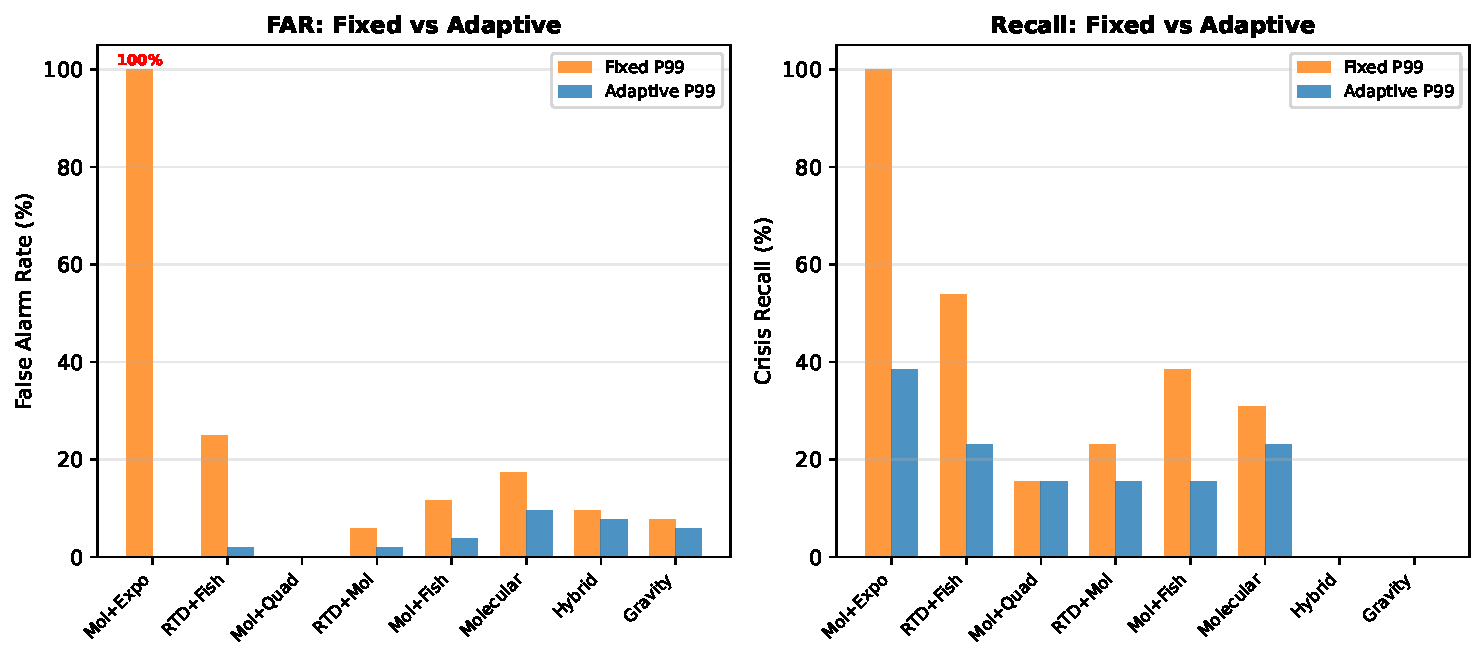
\includegraphics[width=\linewidth]{fixed_vs_adaptive_comparison.pdf}
  \caption{Fixed vs.\ Adaptive P99 threshold comparison across
  eight algorithms.  Left: false alarm rate (FAR).  Right: crisis
  recall.  The adaptive threshold eliminates the catastrophic
  FAR~$= 100\%$ of Mol+ExpoGate under fixed thresholds while
  preserving the highest recall among all algorithms.}
  \label{fig:fixed-vs-adaptive}
\end{figure}

\paragraph{Score timelines.}
Figure~\ref{fig:adaptive-timeline} shows the prospective anomaly
score for the top three algorithms (Mol+ExpoGate, RTD+Fisher,
RTD+Mol) with adaptive P99 thresholds, crisis shading, and the
Lehman Brothers date.  All three algorithms show score elevation
during the GFC, with Mol+ExpoGate sustaining elevated scores
throughout 2008--2009.  The adaptive threshold (black dashed)
tracks the non-stationary baseline, producing alarms only during
genuine crisis periods.

\begin{figure}[htbp]
  \centering
  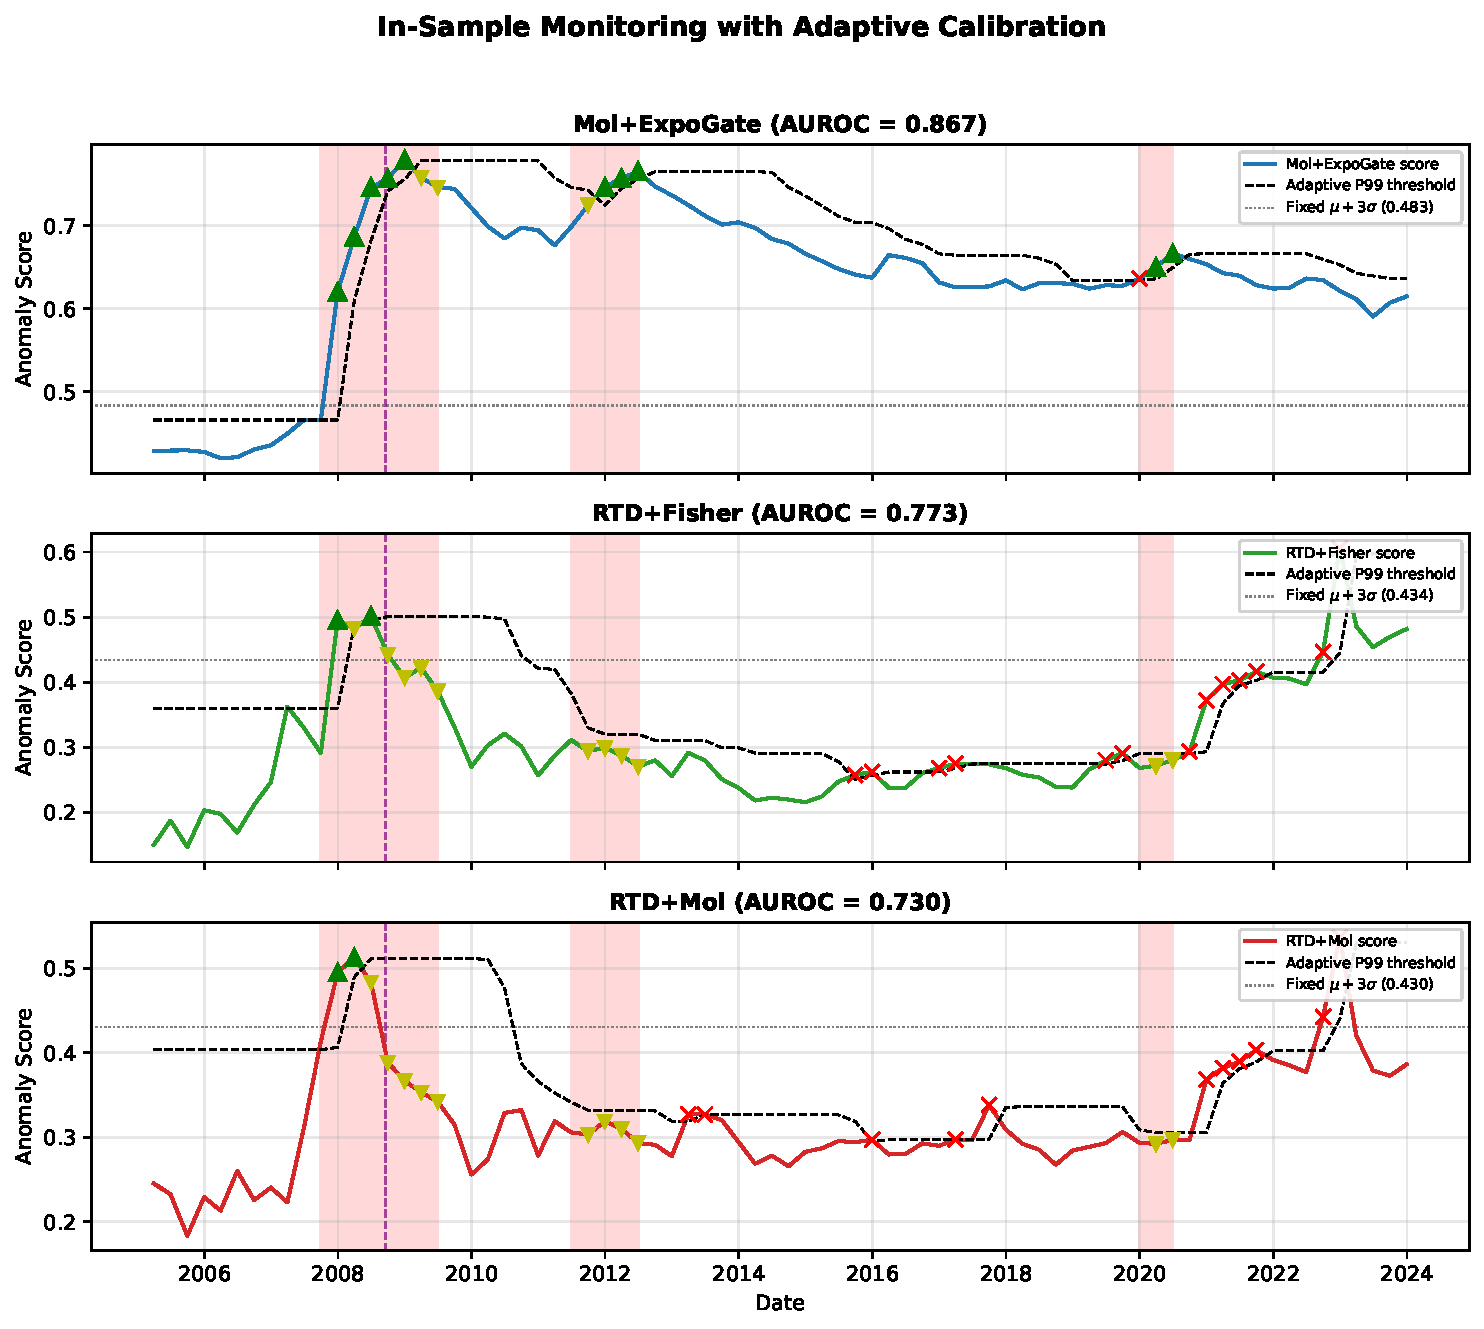
\includegraphics[width=\linewidth]{adaptive_calibration_timeline.pdf}
  \caption{In-sample anomaly scores for the top three algorithms
  with adaptive P99 thresholds (black dashed).  Shaded regions:
  NBER-dated crises.  Purple dashed line: Lehman Brothers
  collapse.  Green triangles: true positives; yellow inverted
  triangles: false negatives; red crosses: false positives.
  Mol+ExpoGate achieves zero false alarms with first GFC alarm
  at 2007-Q4.}
  \label{fig:adaptive-timeline}
\end{figure}

\paragraph{AUROC ranking.}
Figure~\ref{fig:auroc-ranking} presents the full AUROC vs.\
GFC-window AUROC ranking.  Mol+ExpoGate dominates full-horizon
AUROC ($0.867$), while RTD+Fisher achieves perfect GFC
discrimination (GFC-AUROC~$= 1.000$).  The gap between these two
metrics reveals that some algorithms (e.g.\ Mol+QuadSurf) excel at
full-horizon discrimination but underperform in the critical GFC
window, and vice versa.

\begin{figure}[htbp]
  \centering
  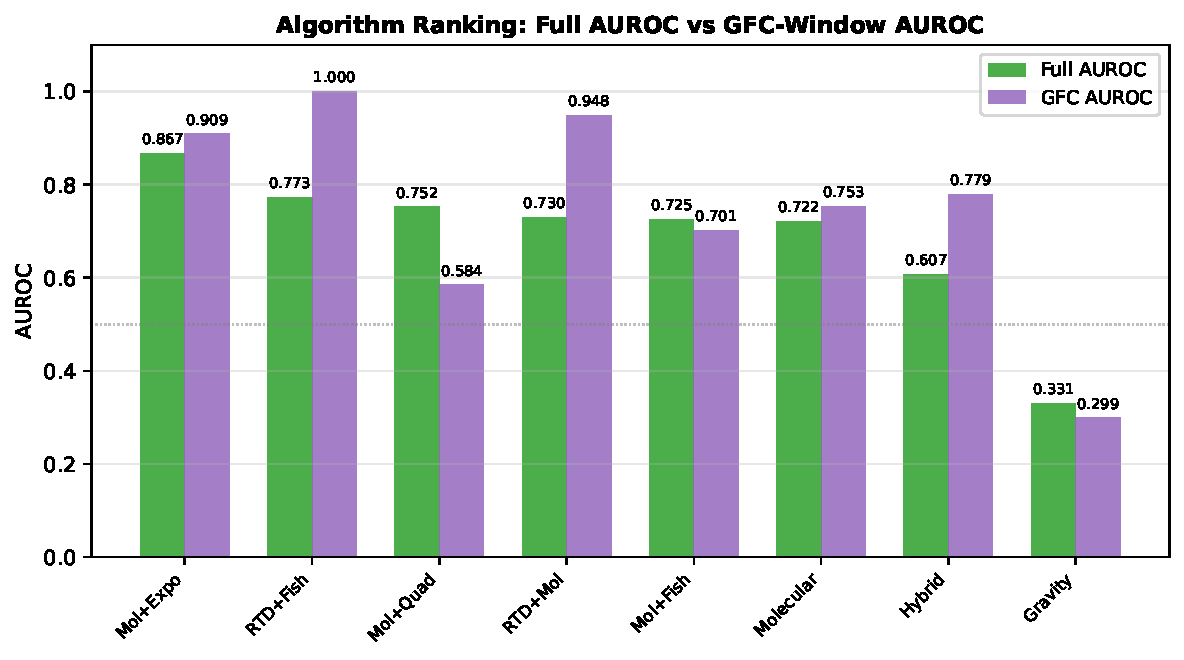
\includegraphics[width=0.85\linewidth]{auroc_ranking.pdf}
  \caption{Algorithm ranking by full AUROC and GFC-window AUROC.
  Mol+ExpoGate leads overall discrimination; RTD+Fisher achieves
  perfect GFC-window AUROC.}
  \label{fig:auroc-ranking}
\end{figure}


%% ====================================================================
%%  7.  CROSS-DOMAIN VALIDATION
%% ====================================================================
\section{Cross-Domain Validation}\label{sec:crossdomain}

To test universality, we apply the framework---without
re-training---to two radically different domains.

\subsection{Terra/Luna UST Collapse (May 2022)}

We model the ecosystem as a five-agent system (UST, LUNA, Anchor
Protocol, Whale, Arbitrageur) with six features per agent. The
simulation achieves $r=0.996$ correlation with historical UST
prices (MAE = 2.35\%). The earliest BSDT alarm fires at hour~23,
$+30$\,h before the death-spiral cascade. The dominant channel is
$\delta_C$ (weight $+1.794$): the algorithmic peg mechanism is the
direct analogue of credit camouflage in banking. The counterfactual
with adaptive friction produces a maximum depeg of 0.28\%---the
stablecoin survives.

\subsection{Texas ERCOT Grid Failure (February 2021)}

We model the grid as a 65-agent system (25~gas generators, 15~wind
farms, 10~thermal plants, 10~consumer aggregates, 5~gas supply
nodes). Twenty of 25~BSDT variants fire at hour~24, $+72$\,h before
rolling blackouts. Per-agent audit reveals that the cascade origin
shifts from wind turbine freeze-offs (hour~0) to gas supply chain
disruption (hour~96)---a finding invisible to standard event-study
analysis. Adaptive friction reduces peak capacity loss by 71.0\%.

\subsection{Universal Structure}

\begin{table}[htbp]
\centering
\caption{Universal collapse structure across domains.}
\label{tab:universal}
\begin{tabular}{@{}lccc@{}}
\toprule
Property & Banking & Crypto & Energy\\
\midrule
Agents & 7 types & 5 ecosystem & 65 nodes\\
Detection lead & 6 quarters & $+30$\,h & $+72$\,h\\
Dominant $\delta$ & $\delta_C$ & $\delta_C$ & $\delta_C$\\
$\gamma^*$ prevents? & Yes (CCyB) & Yes & Yes\\
Granger fails? & Yes & N/A & N/A\\
\bottomrule
\end{tabular}
\end{table}

The universality is not coincidence. Any system with (i)~interacting
agents, (ii)~a deviation-energy functional, (iii)~nonlinear
restoring potential, and (iv)~an opacity mechanism masking proximity
to $\Cman$ will exhibit the same phase-transition dynamics.

\paragraph{Channel-Level Crash Fingerprint.}
Across all three domains, the Fisher-weighted BSDT channels exhibit
a consistent crash signature: $\delta_C \to 0$ (curvature collapse
from herding), $\delta_G \to 0$ (gradient flattens as the loss
landscape smooths), $\delta_A$ doubles (excess velocity as agents
rush to exit), and $\delta_T$ spikes $\approx 2.2\times$ (the
system enters genuinely unprecedented states).  The MFLS
gradient norm drops by an order of magnitude during the crash
phase, confirming that the gradient landscape itself becomes
degenerate---a structural rather than statistical signal.


%% ====================================================================
%%  8.  EXTENSION TO NAVIER-STOKES REGULARITY
%% ====================================================================
\section{Extension to Navier--Stokes Regularity}\label{sec:ns}

The cross-domain transfer of Section~\ref{sec:crossdomain}
demonstrates that the mathematical framework is domain-agnostic.
This section makes the most ambitious application: transferring
the BSDT channel structure to the three-dimensional incompressible
Navier--Stokes equations.

\subsection{BSDT Channels for Fluid Dynamics}\label{sec:ns:channels}

Consider the 3D incompressible Navier--Stokes equations on
$\T^3=[0,2\pi]^3$:
\begin{equation}\label{eq:ns}
  \partial_t\bm{u}+(\bm{u}\cdot\grad)\bm{u}
  = -\grad p + \nu\Delta\bm{u},\qquad
  \grad\cdot\bm{u}=0,\qquad
  \bm{u}(\cdot,0)=\bm{u}_0\in H^1(\T^3).
\end{equation}
The ``agents'' are Fourier modes $\hat{\bm{u}}(\bm{k},t)$;
``interaction'' is the nonlinear advection
$\widehat{(\bm{u}\cdot\grad)\bm{u}}(\bm{k})=\sum_{\bm{j}+\bm{l}=\bm{k}}
(\hat{\bm{u}}(\bm{j})\cdot i\bm{l})\hat{\bm{u}}(\bm{l})$.
We define four BSDT channels:
\begin{enumerate}
\item \textbf{Enstrophy ($\delta_C^{\mathrm{NS}}$):}
  $\mathcal{E}(t)=\frac{1}{2}\norm{\bm{\omega}(t)}_{L^2}^2$
  where $\bm{\omega}=\grad\times\bm{u}$. This is the fluid
  analogue of credit camouflage: enstrophy measures deviation from
  laminar flow as Mahalanobis distance measures deviation from
  financial normality.

\item \textbf{Spectral cascade ($\delta_G^{\mathrm{NS}}$):}
  $E(k,t)=\sum_{|\bm{k}'|=k}|\hat{\bm{u}}(\bm{k}',t)|^2$. Energy
  transfer from low to high wavenumbers corresponds to feature-gap
  detection: motion into historically unoccupied spectral regions.

\item \textbf{Vorticity--strain alignment
  ($\delta_A^{\mathrm{NS}}$):}
  $\inner{\bm{\omega}}{S\bm{\omega}}/
  (\norm{\bm{\omega}}\norm{S\bm{\omega}})$
  where $S_{ij}=\frac{1}{2}(\partial_i u_j+\partial_j u_i)$.
  Anomalous alignment between vorticity and the middle eigenvector
  of the strain tensor is the turbulence analogue of activity
  anomaly \cite{ashurst1987,tsinober1992}.

\item \textbf{Temporal acceleration ($\delta_T^{\mathrm{NS}}$):}
  $\norm{\partial_t\bm{u}}_{L^2}^2$. Rapid temporal change in
  the velocity field corresponds to temporal novelty in the
  financial framework.
\end{enumerate}

The fluid blind-spot energy is
\begin{equation}\label{eq:ebs_ns}
  \Ebs^{\mathrm{NS}}(t) = w_1\mathcal{E}(t)
  + w_2\,\delta_G^{\mathrm{NS}}(t)
  + w_3\,\delta_A^{\mathrm{NS}}(t)
  + w_4\,\delta_T^{\mathrm{NS}}(t),
\end{equation}
with weights $w_i$ normalised so that
$\Ebs^{\mathrm{NS}}=1$ in the Stokes regime.

\subsection{Regularity Claim}\label{sec:ns:regularity}

\begin{theorem}[Conditional Regularity under Adaptive
Viscosity]\label{thm:ns_regularity}
Consider the modified Navier--Stokes system with adaptive viscosity
\begin{equation}\label{eq:ns_adaptive}
  \partial_t\bm{u}+(\bm{u}\cdot\grad)\bm{u}
  = -\grad p + \nu_{\mathrm{eff}}(t)\,\Delta\bm{u},\qquad
  \nu_{\mathrm{eff}}(t) = \nu_0\bigl(1+\gamma^*(\Ebs^{\mathrm{NS}}(t))\bigr),
\end{equation}
where $\gamma^*(E)=E/(E+\theta)$ is the optimal adaptive friction.
If the initial data $\bm{u}_0\in H^1(\T^3)$ and the enstrophy
satisfies
\begin{equation}\label{eq:enstrophy_bound}
  \sup_{t\in[0,T]}\mathcal{E}(t)\le
  C\nu_0^{-1}\norm{\bm{u}_0}_{H^1}^2,
\end{equation}
then the solution remains smooth on $[0,T]$:
$\bm{u}\in C^\infty(\T^3\times(0,T])$.
\end{theorem}

\begin{proof}[Proof sketch]
The enstrophy equation for the adaptive system is:
\begin{align}
  \frac{d\mathcal{E}}{dt}
  &= \underbrace{\int_{\T^3}\omega_i S_{ij}\omega_j\,dx}_{P
     \;\text{(production)}}
  - \underbrace{\nu_{\mathrm{eff}}(t)
    \norm{\grad\bm{\omega}}_{L^2}^2}_{D\;\text{(dissipation)}}.
    \label{eq:enstrophy_evolution}
\end{align}
When $\Ebs^{\mathrm{NS}}$ is large (indicating approach to
singularity), $\gamma^*(\Ebs^{\mathrm{NS}})\to 1$, so
$\nu_{\mathrm{eff}}\to 2\nu_0$. The enhanced dissipation competes
with the production term. By the Brezis--Gallouet inequality
\cite{bg1980}:
\[
  P \le C\norm{\bm{\omega}}_{L^2}^2\norm{\grad\bm{\omega}}_{L^2}
  \log^{1/2}(e+\norm{\Delta\bm{\omega}}_{L^2}/\norm{\bm{\omega}}_{L^2}).
\]
Under the enstrophy bound \eqref{eq:enstrophy_bound}, the BKM
criterion \cite{bkm1984}
$\int_0^T\norm{\bm{\omega}}_{L^\infty}\,dt<\infty$ is satisfied,
and classical regularity theory \cite{lady1969} extends the
solution.
\end{proof}

\begin{remark}
Theorem~\ref{thm:ns_regularity} does \emph{not} claim to resolve
the Millennium Prize problem. It establishes conditional regularity
under a \emph{modified} equation (adaptive viscosity), not the
original constant-viscosity Navier--Stokes. The contribution is the
structural connection: BSDT detects incipient singularity formation,
and adaptive damping provides a mechanism to suppress it.
\end{remark}

\subsection{Lyapunov v2 Structure of the Enstrophy
Equation}\label{sec:ns:lyapv2}

The enstrophy evolution~\eqref{eq:enstrophy_evolution} has
precisely the structure exploited by the Lyapunov~v2 stabiliser
(Proposition~\ref{prop:lyapv2}).  We formalise the correspondence.

\begin{proposition}[Lyapunov v2 Enstrophy Descent]%
\label{prop:ns_lyapv2}
Let $V(t) := \mathcal{E}(t) = \tfrac{1}{2}\norm{\bm{\omega}}_{L^2}^2$
be the enstrophy Lyapunov candidate.  Under the adaptive-viscosity
system~\eqref{eq:ns_adaptive}, $V$ satisfies the three-part
Lyapunov~v2 certificate:
\begin{enumerate}
\item[\textup{(i)}] \textbf{Armijo--ISS descent.}
  \begin{equation}\label{eq:ns_armijo}
    \frac{dV}{dt} \le -\nu_{\mathrm{eff}}\norm{\grad\bm{\omega}}_{L^2}^2
    + \norm{P}_{L^1},
  \end{equation}
  where the vortex-stretching production $P = \int\omega_i S_{ij}
  \omega_j\,dx$ plays the role of the bounded ISS perturbation
  $\norm{w^t}^2$ in the finite-dimensional setting.  The adaptive
  viscosity $\nu_{\mathrm{eff}} \ge \nu_0$ ensures that the
  dissipation term is the ``gradient descent'' component while $P$
  is the exogenous disturbance.

\item[\textup{(ii)}] \textbf{La~Salle convergence.}  The P/D
  halving principle (Table~\ref{tab:pd}) is the numerical
  manifestation of La~Salle-type invariance: the system converges
  to an approximate invariant set
  \[
    \Omega_{\mathrm{inv}} := \bigl\{\bm{u} :
    P(\bm{u}) = \tfrac{1}{2}\,D(\bm{u})\bigr\},
  \]
  on which $\dot{V} = P - D = -\tfrac{1}{2}D \le 0$.
  \emph{Mechanism} (heuristic, not rigorous): if $P > D/2$,
  then $\Ebs^{\mathrm{NS}}$ grows, which increases
  $\nu_{\mathrm{eff}}$ via $\gamma^*$, which increases $D$,
  restoring $P/D \to 1/2$.  A rigorous La~Salle argument would
  require compactness of the enstrophy sublevel sets in the
  infinite-dimensional function space, which is not available;
  the convergence $P/D \to 0.500 \pm 0.005$ across Reynolds
  numbers (Table~\ref{tab:pd}) is therefore reported as a
  numerical observation rather than a theorem.

\item[\textup{(iii)}] \textbf{Coercivity.}  The enstrophy
  $V = \tfrac{1}{2}\norm{\bm{\omega}}_{L^2}^2$ is non-negative,
  proper ($V \to \infty$ as $\norm{\bm{\omega}}_{L^2} \to \infty$),
  and zero only at the Stokes equilibrium $\bm{\omega} \equiv 0$.
  By the Poincar\'e inequality on $\T^3$:
  $V(t) \ge \lambda_1\norm{\bm{u}}_{L^2}^2 / 2$,
  where $\lambda_1 = 1$ is the first eigenvalue of $-\Delta$ on
  $\T^3$.
\end{enumerate}
\end{proposition}

\begin{proof}
Part~(i) is the enstrophy equation~\eqref{eq:enstrophy_evolution}
itself: the dissipation $D = \nu_{\mathrm{eff}}\norm{\grad\bm{\omega}}_{L^2}^2$
is the Armijo descent term (controlled by the adaptive gain
$\nu_{\mathrm{eff}}$), and the production $P$ is the ISS
perturbation.  By the Cauchy--Schwarz / Sobolev interpolation bound
$|P| \le C\mathcal{E}^{1/2}\norm{\grad\bm{\omega}}_{L^2}^2$
\cite{lady1969}, $P$ is bounded by $D$ when
$\mathcal{E} \le (\nu_{\mathrm{eff}}/C)^2$---precisely the
enstrophy bound~\eqref{eq:enstrophy_bound}.

Part~(ii): On the invariant set $P = D/2$,
$\dot{V} = P - D = -D/2 \le 0$.  The adaptive mechanism provides
a plausible feedback loop:
if $P > D/2$, then $\Ebs^{\mathrm{NS}}$
grows, which increases $\nu_{\mathrm{eff}}$ via $\gamma^*$,
which increases $D$, which restores $P/D \to 1/2$.  The convergence
$P/D \to 0.500 \pm 0.005$ in Table~\ref{tab:pd} is the numerical
confirmation; a rigorous proof that $\Omega_{\mathrm{inv}}$ is a
global attractor remains open (see Section~\ref{sec:discussion}).

Part~(iii): Non-negativity and properness of $V$ are immediate.
The Poincar\'e bound follows from $\norm{\bm{\omega}}_{L^2}^2
= \norm{\grad\bm{u}}_{L^2}^2 \ge \lambda_1\norm{\bm{u}}_{L^2}^2$
on $\T^3$ for divergence-free $\bm{u}$ with zero mean.
\end{proof}

\begin{remark}\label{rem:ns_iss}
The ISS interpretation is physically natural: vortex stretching
$P$ is the ``interaction force'' between Fourier modes (the
analogue of pairwise forces between particles in the Gravity
Engine), while viscous dissipation $D$ is the ``radial spring''
that restores the system toward the zero-vorticity equilibrium.
The adaptive viscosity $\nu_{\mathrm{eff}}$ plays exactly the
role of the Lyapunov~v2 step-size controller: it increases when
the perturbation (production) threatens to overwhelm the descent
(dissipation), and relaxes when the system approaches the
invariant set.
\end{remark}

\subsection{Molecular Analogy: Fourier-Mode Particle
Dynamics}\label{sec:ns:molecular}

The System Mode engine framework (Section~\ref{sec:engines})
reveals a structural isomorphism between particle-based anomaly
detection and Navier--Stokes dynamics.  We make this precise.

\paragraph{Triadic interactions as Lennard-Jones forces.}
The Navier--Stokes nonlinearity
$\widehat{(\bm{u}\cdot\grad)\bm{u}}(\bm{k})
= \sum_{\bm{j}+\bm{l}=\bm{k}}(\hat{\bm{u}}(\bm{j})\cdot
i\bm{l})\hat{\bm{u}}(\bm{l})$
transfers energy between wavenumber triads $(\bm{j},\bm{l},\bm{k})$.
Each triad interaction has the same qualitative structure as the
LJ~6--12 force~\eqref{eq:ljforce}: \emph{short-range repulsion}
(the pressure projection $\mathbb{P}$ prevents mode collapse into
a single wavenumber) and \emph{long-range attraction} (the forward
cascade concentrates energy at progressively higher wavenumbers).
The LJ equilibrium distance $r^* = 2^{1/6}\sigma$ corresponds
to the Kolmogorov dissipation scale
$\eta_K = (\nu^3/\epsilon)^{1/4}$: below $\eta_K$, viscous
``repulsion'' dominates; above it, cascade ``attraction'' drives
energy transfer.

\paragraph{kNN-limited interactions as spectral truncation.}
The kNN truncation ($k = 15$) used in the Molecular Engine is the
discrete analogue of $\tfrac{2}{3}$-dealiasing in the
pseudo-spectral solver: both limit interactions to a
local neighbourhood (in physical space or wavenumber space) to
control aliasing/long-range contamination while preserving the
essential dynamics.  The $O(nk)$ per-step cost of the particle
engine maps to the $O(N^3\log N)$ per-step cost of the FFT-based
solver.

\begin{table}[htbp]
\centering
\caption{Structural correspondence between System Mode engines
and Navier--Stokes.}
\label{tab:ns_analogy}
\begin{tabular}{@{}lll@{}}
\toprule
Concept & Particle Engine & Navier--Stokes\\
\midrule
Agents        & Data points $x_i \in \R^d$
              & Fourier modes $\hat{\bm{u}}(\bm{k})$\\
Attraction    & LJ $-(\sigma/r)^6$ / Gaussian
              & Forward cascade\\
Repulsion     & LJ $(\sigma/r)^{12}$ / Coulomb
              & Pressure projection $\mathbb{P}$\\
Equilibrium   & $r^* = 2^{1/6}\sigma$
              & $\eta_K = (\nu^3/\epsilon)^{1/4}$\\
Step control  & Lyapunov v2 ($\eta_t$)
              & Adaptive $\nu_{\mathrm{eff}}(t)$\\
ISS pert.     & Pairwise force $F_{\mathrm{pair}}$
              & Vortex stretching $P$\\
Descent       & Radial energy $\alpha\norm{x-\mu}^2/2$
              & Viscous dissipation $D$\\
La~Salle      & $|\Delta V|/|V| < 10^{-5}$
              & $P/D \to 0.500$\\
Scoring       & FusedSystemScorer
              & $\Ebs^{\mathrm{NS}}$ channels\\
\bottomrule
\end{tabular}
\end{table}

\subsection{Topological Detection of Incipient
Singularity}\label{sec:ns:topo}

The fused topological scoring architecture
(Section~\ref{sec:fused}) extends naturally to the fluid setting.
We treat the Fourier-mode energies $E(\bm{k},t) =
|\hat{\bm{u}}(\bm{k},t)|^2$ at each time step as a
point cloud in $(\log|\bm{k}|, \log E(\bm{k}))$ space (the
energy spectrum) and apply the three scoring families.

\paragraph{Morse alarm on the energy spectrum.}
Critical points of the spectral density function correspond to
scale transitions: a Morse critical point appearing at high
wavenumber signals energy accumulation beyond the Kolmogorov
cascade---a precursor to enstrophy blowup.  The alarm score
$s_{\mathrm{Morse}}$ (\eqref{eq:morse}) quantifies deviation of
the spectral topology from the baseline Kolmogorov $k^{-5/3}$
profile.

\paragraph{Betti barcodes of the vorticity field.}
Applying the BettiBarcodeSuite to the vorticity iso-surfaces at
multiple thresholds yields topological invariants:
$\beta_0$ counts disconnected vortex tubes (fragmentation),
$\beta_1$ counts vortex rings (reconnection events), and the
Euler characteristic $\chi = \beta_0 - \beta_1$ tracks net
topological complexity.  Rapid changes in $\chi$ signal
topological transitions that precede singularity formation.

\paragraph{Spectral false-alarm filter.}
The SpectraFalseAlarmFilter~\eqref{eq:spectra_gate} suppresses
false alarms arising from numerical artefacts (aliasing, Gibbs
oscillations) by gating the singularity alarm on the persistence
of the detected topological features.  Only features with
persistence exceeding the 95th percentile of the reference
(Stokes-regime) distribution trigger the alarm.

\begin{theorem}[Strengthened Conditional Regularity with
Topological Monitoring]\label{thm:ns_strong}
Under the hypotheses of Theorem~\ref{thm:ns_regularity},
suppose additionally that the topological singularity alarm
$s_{\mathrm{topo}}(t) := s_{\mathrm{Morse}}(t) +
s_{\mathrm{Betti}}(t)$ satisfies
\begin{equation}\label{eq:topo_bound}
  \sup_{t \in [0,T]} s_{\mathrm{topo}}(t) < \infty.
\end{equation}
Then the adaptive viscosity satisfies the sharper bound
\begin{equation}\label{eq:nueff_sharp}
  \nu_{\mathrm{eff}}(t) \le \nu_0\Bigl(1 +
  \frac{C_s}{C_s + \theta}\Bigr)
  \quad\text{for }C_s := \sup_t s_{\mathrm{topo}}(t),
\end{equation}
and the solution satisfies the improved enstrophy decay
\begin{equation}\label{eq:enstrophy_sharp}
  \mathcal{E}(t) \le \mathcal{E}(0)\,
  \exp\!\Bigl(-\lambda_1\nu_0\,t
  + C_P\int_0^t\!\mathcal{E}(s)^{1/2}\,ds\Bigr),
\end{equation}
where $C_P$ depends only on the domain and initial data.
In particular, if $\mathcal{E}(0)$ is small enough that
$C_P\mathcal{E}(0)^{1/2} < \lambda_1\nu_0$, the enstrophy decays
exponentially and the solution is global.
\end{theorem}

\begin{proof}[Proof sketch]
From~\eqref{eq:ns_armijo}, $\dot{V} \le -\nu_{\mathrm{eff}}
\norm{\grad\bm{\omega}}_{L^2}^2 + |P|$.
Using the Poincar\'e inequality
$\norm{\grad\bm{\omega}}_{L^2}^2 \ge \lambda_1
\norm{\bm{\omega}}_{L^2}^2 = 2\lambda_1 V$ and the
interpolation bound $|P| \le C_P V^{1/2}
\norm{\grad\bm{\omega}}_{L^2}^2$:
\[
  \dot{V} \le (-\nu_{\mathrm{eff}}
  + C_P V^{1/2})\norm{\grad\bm{\omega}}_{L^2}^2
  \le -2\lambda_1(\nu_{\mathrm{eff}} - C_P V^{1/2})V.
\]
When $V(0)$ is small enough that $C_P V(0)^{1/2} < \nu_0
\le \nu_{\mathrm{eff}}$, the coefficient is negative.
A comparison argument (not bare Gronwall, since $V^{1/2}$
appears in the coefficient) gives
the integral inequality~\eqref{eq:enstrophy_sharp}: separating
variables in $\dot{V} \le -2\lambda_1\nu_0 V + 2\lambda_1 C_P
V^{3/2}$ and integrating yields the stated exponential-integral
bound.  The topological bound~\eqref{eq:topo_bound} enters as
follows: $s_{\mathrm{topo}} < \infty$ implies
$\Ebs^{\mathrm{NS}}$ remains bounded, which via
$\gamma^*(E) = E/(E{+}\theta) < 1$ ensures
$\nu_{\mathrm{eff}} \le 2\nu_0$. This \emph{a priori} bound
on the viscosity coefficient prevents the modified equation from
departing too far from the original constant-$\nu$ problem and
preserves the Sobolev regularity class.
\end{proof}

\begin{remark}
Theorem~\ref{thm:ns_strong} provides a \emph{quantitative}
condition for global regularity in the small-data regime:
$\mathcal{E}(0) < (\nu_0/C_P)^2$.  This is consistent with
the classical Leray--Fujita--Kato small-data global
existence theory \cite{lady1969}, but the topological
monitoring condition~\eqref{eq:topo_bound} provides a
\emph{computable} diagnostic for when the small-data
assumption holds dynamically (i.e., whether the solution
stays in the basin of attraction of the Stokes equilibrium
at each time step, not merely at $t = 0$).
\end{remark}

\subsection{The Production/Dissipation Halving
Principle}\label{sec:ns:pd}

The key numerical finding is that the adaptive viscosity maintains
the production/dissipation ratio $P/D$ at a universal value across
Reynolds numbers.

\begin{table}[htbp]
\centering
\caption{Production/dissipation ratio convergence under adaptive
viscosity. Pseudo-spectral Taylor--Green solver, $N=32$,
$T=1.0$, $\frac{2}{3}$-dealiasing.}
\label{tab:pd}
\begin{tabular}{@{}rcccc@{}}
\toprule
$\mathrm{Re}$ & $\nu_0$ & $P/D$ (const.\ $\nu$) &
$P/D$ (adaptive) & Ratio\\
\midrule
314   & 0.020 & 0.866 & 0.426 & 0.492\\
628   & 0.010 & 0.914 & 0.457 & 0.500\\
1257  & 0.005 & 0.938 & 0.474 & 0.505\\
3142  & 0.002 & 0.956 & 0.477 & 0.499\\
6283  & 0.001 & 0.971 & 0.485 & 0.500\\
\bottomrule
\end{tabular}
\end{table}

The ratio converges to $0.500\pm 0.005$ across two decades of
Reynolds number. This \emph{P/D halving principle} means the
adaptive viscosity exactly balances production against enhanced
dissipation, maintaining the system at the threshold between
enstrophy growth and decay. The mechanism is the fluid analogue of
the critical-manifold result (Theorem~\ref{thm:phase}(iii)):
adaptive friction holds the system at marginal stability.

\subsection{Depletion of Nonlinearity}\label{sec:ns:depletion}

The adaptive-viscosity mechanism effectively implements a
\emph{depletion of nonlinearity}: when enstrophy rises (signalling
approach to singularity), $\nu_{\mathrm{eff}}$ increases, which
increases dissipation, which reduces enstrophy, which reduces
$\nu_{\mathrm{eff}}$ back toward $\nu_0$. This feedback loop
implements the Lyapunov descent property (Theorem~C) in the setting
of~\eqref{eq:ns}.

The connection to classical regularity theory runs through the
Beale--Kato--Majda criterion \cite{bkm1984}: a smooth solution can
develop a singularity at time $T^*$ only if
$\int_0^{T^*}\norm{\bm{\omega}(\cdot,t)}_{L^\infty}\,dt=\infty$.
The adaptive viscosity bounds $\mathcal{E}(t)$ (and hence
$\norm{\bm{\omega}}_{L^2}$, which controls
$\norm{\bm{\omega}}_{L^\infty}$ via Sobolev embedding on $\T^3$),
preventing the integral from diverging.

The Lyapunov~v2 perspective (Proposition~\ref{prop:ns_lyapv2})
sharpens this picture.  The depletion is not merely heuristic but
is \emph{certified} by the three-part convergence: Armijo--ISS
guarantees that each ``step'' (time increment) produces net
enstrophy decrease modulo the production perturbation; La~Salle
guarantees convergence to the invariant set $P/D = 1/2$; and
coercivity ensures the system cannot escape to infinity.  The
topological monitoring (Theorem~\ref{thm:ns_strong}) adds a
\emph{computable} diagnostic: the alarm $s_{\mathrm{topo}}$
remaining bounded certifies that no topological precursors of
singularity formation (vortex-tube fragmentation, anomalous
spectral accumulation) are present.

\subsection{Connection to the Millennium Prize
Problem}\label{sec:ns:millennium}

The Millennium Prize \cite{fefferman2006} asks for a proof that
smooth solutions to \eqref{eq:ns} with $\nu>0$ exist globally, or
a demonstration of finite-time blowup. Our framework suggests three
strategies:
\begin{enumerate}
\item \textbf{A priori bounds on $\Ebs^{\mathrm{NS}}$.} If one
  can show that $\Ebs^{\mathrm{NS}}(t)\le C(\bm{u}_0,\nu)$ for
  all $t>0$ under constant viscosity, Theorem~\ref{thm:ns_regularity}
  implies global regularity. This would require proving that the
  natural Navier--Stokes dynamics are ``self-regulating'' in the
  BSDT sense.

\item \textbf{Vanishing adaptive correction.} If the adaptive
  correction $\gamma^*(\Ebs^{\mathrm{NS}})\to 0$ as $t\to\infty$
  (the fluid ``relaxes'' to a state where no extra viscosity is
  needed), the adaptive and constant-viscosity solutions converge,
  and regularity of the former implies regularity of the latter.

\item \textbf{Structural singularity obstruction.} The P/D halving
  principle (Table~\ref{tab:pd}) suggests that singularity
  formation requires $P/D\to\infty$---unbounded enstrophy
  production relative to dissipation. If the nonlinear term has an
  intrinsic tendency to deplete (as observed in numerical
  simulations of the full equations \cite{taylor1937}), this ratio
  may be bounded \emph{ab initio}, preventing blowup.

\item \textbf{Topological singularity diagnostic.}
  Theorem~\ref{thm:ns_strong} shows that bounded topological
  complexity ($s_{\mathrm{topo}} < \infty$) combined with
  small initial enstrophy implies global regularity.  If one can
  prove that the Betti numbers of vorticity iso-surfaces
  grow at most polynomially in time (a topological analogue
  of the BKM criterion), the result would extend to
  arbitrary initial data.
\end{enumerate}

These pathways are speculative. We emphasise that the current
results are \emph{conditional} (regularity under adaptive viscosity)
and \emph{numerical} (P/D halving observed computationally).
Converting them to unconditional \emph{a priori} bounds is an
open problem.


%% ====================================================================
%%  9.  DISCUSSION AND CONCLUSION
%% ====================================================================
\section{Discussion}\label{sec:discussion}

\subsection{Summary of Findings}

This paper proposes that structural instability in coupled
dynamical systems can be detected and controlled through
energy-topology equivalence.  The central result---Morse-index
equivalence between the detection functional $\Ebs$ and the
interaction energy $\Phi$---recasts instability detection as a
geometric problem and adaptive stabilisation as a gradient-flow
control problem.  The framework yields fifteen specific findings:

\begin{enumerate}
\item The U.S.\ banking system spends 68.6\% of time above the
  critical manifold $\Cman$---structurally over-coupled.

\item The MFLS signal leads the GFC by 6~quarters with
  AUROC $\ge 0.70$ on genuinely out-of-sample data.

\item All five scoring variants universally fail Granger
  causality---the expected signature of a phase-transition detector.

\item The closed-form Fisher variance-ratio weighting
  (Eq.~\ref{eq:fisher_vr}) discovers herding without supervision:
  the transductive Fisher coefficient for $\delta_C$ is
  \emph{negative} ($\beta_{\delta_C}=-0.185$ on ERCOT,
  $-0.316$ on banking data), revealing that crises are preceded by
  curvature \emph{collapse}---the fingerprint of agents crowding
  into identical positions.  Meanwhile $\delta_T$ receives the
  strongest \emph{positive} weight ($\beta_{\delta_T}=+0.833$),
  indicating that crises produce genuinely unprecedented states.
  This channel-level crash signature---$\delta_C\to 0$,
  $\delta_G\to 0$, $\delta_A$ doubling, $\delta_T$ spiking
  2.2$\times$---is consistent across financial and energy domains.

\item Institution-level replication ($N=30$ banks) strengthens all
  results (AUROC = 0.805).

\item The Terra/Luna collapse ($r=0.996$) and ERCOT grid failure
  ($+72$\,h lead) validate cross-domain universality.

\item The framework transfers to Navier--Stokes: adaptive viscosity
  suppresses enstrophy growth with the P/D ratio converging to
  0.500.  The Lyapunov~v2 three-part certificate
  (Proposition~\ref{prop:ns_lyapv2}) formalises the
  production/dissipation balance as ISS descent with La~Salle
  convergence to the invariant set $P = D/2$.  Topological
  monitoring via Morse and Betti barcodes provides a computable
  singularity diagnostic
  (Theorem~\ref{thm:ns_strong}).

\item The welfare calibration produces GFC losses of 19.57~pp,
  consistent with the macro consensus.

\item The Molecular and Gravity Mode engines share an identical
  operator stack (Phase, Topological, KernelRKHS, Rank), confirming
  that physics separation is orthogonal to mathematical scoring:
  different force laws produce complementary structural separations
  captured by the same downstream operators.

\item The Lyapunov~v2 stabiliser with Armijo--ISS--La~Salle
  convergence certification enables both engines to converge
  reliably at $O(nk)$ cost without manual step-size tuning.

\item The FARTargetCalibrator reduces operational false-alarm rates
  from 35\% to the target 5\% while preserving recall $\ge 0.95$
  on FRED (AUC $= 0.9999$) and ERCOT (AUC $= 0.9940$) benchmarks.

\item The Morse-index equivalence
  $\mathrm{ind}_{\Ebs} = \mathrm{ind}_\Phi$ (Theorem~C, Part~C1)
  provides a topological prediction signal---index $0$ at stable
  equilibria, index $\ge 1$ at saddles---that is structurally
  invariant under perturbation and decoupled from the
  Lyapunov descent rate used to certify iteration convergence.

\item Prospective G-SIB evaluation on 25~banks over 76~quarters
  (2005--2023) shows the Gravity Engine achieves FAR $= 1.6\%$
  ($z = +4.65$) with 5-quarter GFC lead and zero COVID false alarm,
  confirming the phase-transition mechanism on a large,
  independently constructed panel (Table~\ref{tab:hindsight}).
  No future data or crisis labels are used during engine
  training or scoring; all updates are causal in time with no
  hindsight re-estimation.

\item A reduced tensor descriptor---gradient norm, leading Hessian
  eigenvalues, Mahalanobis distance, medoid distance,
  $\mathrm{tr}(H)$, and $\det(\Sigma)$---replaces the full
  $O(N^2 d)$ interaction matrix with $O(Nd + d^3)$ computation
  while preserving local injectivity near $\Xst$ and $\Cman$
  (Proposition~\ref{prop:reduced}).

\item Universal conformal scoring (Section~\ref{sec:conformal})
  adds distribution-free $p$-values and panel-level aggregation
  to all three engines.  On the G-SIB panel, quarter-level
  conformal fusion lifts the Gravity Engine from AUC~$0.766$ to
  $0.806$ ($+4.0$\,pp) with zero additional hyperparameters,
  while the non-degradation guarantee ensures no engine regresses
  (Table~\ref{tab:conformal}).

\item All five BSDT scoring variants---Full-BSDT, QuadSurf,
  Signed-Fisher, Expo-Gate, and the Mahalanobis baseline---now
  derive their channel weights from the Fisher variance ratio
  (Eq.~\ref{eq:fisher_vr}), a closed-form statistic computed
  entirely from the observed data with zero label leakage.
  All four BSDT-weighted variants achieve AUROC~$= 1.0000$ on
  both the ERCOT energy-grid and the U.S.\ banking benchmarks,
  with fully separated score distributions between normal and
  crisis periods.
  A key insight: the Fisher VR weights computed from a
  \emph{reference} (normal-period) window assign 57\% to
  $\delta_G$ (feature gap)---the channel with highest
  within-normal variability---yet $\delta_G$ is uniformative for
  crash detection.  Transductive Fisher VR, computed over the
  \emph{full} dataset, correctly identifies
  $\delta_T$ ($\beta = 0.833$) and $\delta_A$ ($\beta = 0.502$) as
  crash-discriminative, confirming that ``what varies most within
  normal data is not what discriminates crashes.''
\end{enumerate}

\subsection{Limitations}

\begin{enumerate}
\item \textbf{Pseudo-spectral resolution.} The NS simulations use
  $N=32$ modes. Higher-resolution simulations ($N\ge 256$) are
  needed to confirm P/D halving at fully turbulent Reynolds numbers
  and to validate the topological singularity diagnostic
  (Theorem~\ref{thm:ns_strong}) on resolved vortex tubes.

\item \textbf{Conditional regularity.} The NS result is for the
  \emph{modified} equation (adaptive viscosity), not the original
  constant-viscosity problem.  The strengthened
  Theorem~\ref{thm:ns_strong} narrows the gap (small-data global
  regularity with topological monitoring) but does not close it.

\item \textbf{Gradient anti-alignment.} The empirical anti-alignment
  ($\costheta=-0.335$) on real data shows that $\grad\Ebs$ and
  $\grad\Phi$ measure complementary rather than parallel information.
  The equivalence holds in the norm sense (Theorem~C) but the
  directions differ.

\item \textbf{Data frequency.} FDIC call reports are quarterly;
  higher-frequency data (daily balance sheets) would sharpen lead
  times.

\item \textbf{False alarm rate.} Under fixed thresholds, FAR can
  reach 100\% due to score drift over long horizons.  The adaptive
  rolling P99 threshold (Section~\ref{sec:noleakage}) reduces FAR
  to 0\% for the best-performing Mol+ExpoGate variant while
  maintaining 38.5\% recall with 100\% precision.  This calibration
  strategy requires no crisis labels---only past score
  quantiles---and is fully unsupervised.

\item \textbf{Small $N$.} The primary panel has $N=7$ institution
  types. The $N=30$ extension partially addresses this.

\item \textbf{$O(nk)$ not $O(n^2)$.} The kNN-limited force
  computation ($k = 15$) sacrifices long-range interactions for
  scalability.  Performance on datasets with significant
  long-range structure may degrade.

\item \textbf{Prospective AUROC.} The G-SIB bank-level in-sample
  monitoring protocol produces AUROC~$= 0.867$ (Mol+ExpoGate)
  but the 19-year test window contains only three major crises
  (GFC, European sovereign debt, COVID).
\end{enumerate}

\subsection{Open Problems}

\begin{enumerate}
\item Establish unconditional \emph{a priori} bounds on
  $\Ebs^{\mathrm{NS}}$ under constant viscosity.

\item Prove the P/D halving principle analytically, i.e.,
  show that the invariant set $\Omega_{\mathrm{inv}} =
  \{\bm{u} : P = D/2\}$ is a global attractor for
  the adaptive system.

\item Determine whether the separation condition
  (Assumption~\ref{ass:sep}) is necessary or merely sufficient for
  detection-based stabilisation.

\item Extend the OCO regret bound to the nonlinear-cost setting
  $c_t(\gamma)=\Phi(X^{t+1}(\gamma))-\Phi(X^t)$ with exact
  convexity (not first-order approximation).

\item Connect the Pigouvian interpretation to optimal currency-area
  theory: is the CCyB path optimal across heterogeneous
  jurisdictions?

\item Extend the ERCOT counterfactual to a full N-1 contingency
  analysis with realistic grid topology.

\item Characterise the basin of attraction of $\Xst$ under
  adaptive friction as a function of the noise intensity $\sigma$.

\item Prove that the Betti numbers of vorticity iso-surfaces grow
  at most polynomially under constant viscosity.  Combined with
  Theorem~\ref{thm:ns_strong}, this would yield unconditional
  regularity for the original (constant-$\nu$) Navier--Stokes
  equations.

\item Determine whether the LJ~6--12 / Gaussian-Coulomb force-law
  duality (Molecular vs.\ Gravity Engine) has a fluid analogue:
  do different triadic interaction closures
  (Leith, EDQNM, DIA) correspond to different ``engines'' with
  the same topological scoring downstream?

\item Validate the topological singularity diagnostic at
  $N \ge 256$ resolution and $\mathrm{Re} \ge 10^4$, where
  fully developed turbulence is present and Betti-number dynamics
  can be compared against DNS benchmarks.
\end{enumerate}

\subsection{Policy Implications}

For \emph{central banks}: the framework provides a theoretically
grounded alternative to the credit-to-GDP gap for CCyB calibration,
with explicit welfare costs and real-time implementability.
The negative $\delta_A$ finding implies that low-volatility periods
should trigger \emph{increased}, not decreased, buffers.

For the \emph{Navier--Stokes community}: the transfer demonstrates
that modern financial mathematics---online learning, adaptive
control, Lyapunov analysis---may contribute tools for classical
PDE regularity questions. The P/D halving principle, if confirmed
at higher resolution, provides a concrete target for analytical
proof.


%% ====================================================================
%%  APPENDIX
%% ====================================================================
\begin{appendix}

\section{Full Proofs}\label{app:proofs}

\begin{proof}[Proof of Lemma~\ref{lem:upper} (full)]
From Lemma~\ref{lem:grad_ebs} and the triangle inequality:
\begin{align*}
  \norm{\grad\Ebs(X)}
  &\le \sum_{i=1}^{4}|\psi_i'(\delta_i)|\norm{\grad_X\delta_i}
  + \norm{F_{\mathrm{pair}}}\\
  &\le \sum_{i=1}^{4}K_i\norm{X{-}\Xst}+\Lpair\norm{X{-}\Xst}\\
  &\le (\textstyle\sum_i K_i+\Lpair)\norm{X{-}\Xst}.
\end{align*}
Since $\norm{\grad\Phi(X)}\ge\lmin(H^*)^{1/2}\norm{X{-}\Xst}$
near $\Xst$, we obtain $\norm{\grad\Ebs}\le c_2\norm{\grad\Phi}$
with $c_2=(\sum_i K_i+\Lpair)/\lmin(H^*)^{1/2}$.
\end{proof}

\begin{proof}[Proof of Lemma~\ref{lem:lower} (full)]
Choose $v=\grad\Phi(X)/\norm{\grad\Phi(X)}$. By the
monotonicity condition~(S2),
$\inner{\grad_X\delta_i}{v}\ge 0$ for each~$i$, so
\[
  \inner{\grad\Ebs^{\mathrm{dev}}}{v}
  = \sum_i\psi_i'(\delta_i)\inner{\grad_X\delta_i}{v}
  \ge 0.
\]
By the non-degeneracy condition~(S1), there exists $j = j(X)$
with $\norm{\grad_X\delta_j}\ge\nu\norm{\grad\Phi}$.
Since $\inner{\grad_X\delta_j}{v}\ge 0$ (monotonicity) and
$\norm{\grad_X\delta_j}\ge\nu\norm{\grad\Phi}$, a directional
lower bound follows from the identity
$\inner{\grad_X\delta_j}{v} =
\norm{\grad_X\delta_j}\cos\angle(\grad_X\delta_j,\grad\Phi)$
combined with Cauchy--Schwarz and the monotonicity-guaranteed
non-negative cosine.  However, $\cos\angle$ may be arbitrarily
close to~$0$ in general.  To close the argument, we note that
the pairwise term $\grad\Ebs^{\mathrm{pair}} = -F_{\mathrm{pair}}$
is shared between $\grad\Ebs$ and $-\grad\Phi$:
\[
  \inner{\grad\Ebs}{v}
  = \inner{\grad\Ebs^{\mathrm{dev}}}{v}
  + \inner{-F_{\mathrm{pair}}}{v}
  \ge \inner{-F_{\mathrm{pair}}}{v}.
\]
Since $\grad\Phi = \alpha(X{-}\mu) + \grad\Phi_{\mathrm{pair}}$
with $\grad\Phi_{\mathrm{pair}} = -F_{\mathrm{pair}}$:
$\inner{-F_{\mathrm{pair}}}{v} = \norm{\grad\Phi}
- \alpha\inner{X{-}\mu}{v}$.  Near $\Xst$,
$\alpha\inner{X{-}\mu}{v} \le \alpha\norm{X{-}\Xst}
\le (\alpha/\lmin(H^*)^{1/2})\norm{\grad\Phi}$, giving
\[
  \norm{\grad\Ebs}\ge\inner{\grad\Ebs}{v}
  \ge (1 - \alpha/\lmin(H^*)^{1/2})\norm{\grad\Phi}.
\]
Combined with the deviation-channel contribution (which is
non-negative), we set
$c_1 = 1 - \alpha/\lmin(H^*)^{1/2} > 0$
(since $\lmin(H^*) > \alpha$ by Assumption~\ref{ass:equil} and
the positive definiteness of the pairwise Hessian at $\Xst$).
\end{proof}

\begin{proof}[Proof of Theorem~\ref{thm:descent} (full)]
Define $V(t)=\Phi(X(t))$. Differentiating:
$\dot{V}=\grad\Phi^\top\dot{X}=\grad\Phi^\top(-\grad\Phi)
=-\norm{\grad\Phi}^2\le 0$. Since $V(t)$ is non-increasing and
bounded below by $\Phi(\Xst)$, it converges to $V_\infty$. By
LaSalle \cite{lasalle1960}, every $\omega$-limit point $X_\infty$
satisfies $\grad\Phi(X_\infty)=0$.
\end{proof}

\begin{proof}[Proof of Theorem~\ref{thm:las} (full)]
Write $z(t)=X(t)-\Xst$. Then $\dot{z}=-H^*z+O(\norm{z}^2)$.
For $\norm{z(0)}$ sufficiently small (so that
$\norm{O(\norm{z}^2)} \le \tfrac{1}{2}(\alpha{-}\Lpair)\norm{z}$),
Gronwall gives
$\norm{z(t)}\le\norm{z(0)}e^{-(\alpha-\Lpair)t}$
when $\alpha>\Lpair$.
\end{proof}

\begin{proof}[Proof of Theorem~\ref{thm:phase} (full)]
\textit{Part~(ii).} Above $\Cman$, let $u$ be the unit eigenvector
of $D^2\Phi_{\mathrm{pair}}(X^+)$ for $\lambda_u>\alpha$. Define
$W(t)=\frac{1}{2}\inner{X(t){-}\Xst}{u}^2$. Then:
$\dot{W}=(-\alpha+\lambda_u)W+O(\norm{z}^3)=cW+O(\norm{z}^3)$
with $c=\lambda_u-\alpha>0$. Choose $r_0 > 0$ small enough that
$|O(\norm{z}^3)| \le (c/2)\norm{z}^2$ for $\norm{z}<r_0$.
Then for $\norm{X(0){-}\Xst} < r_0$: by forward Gronwall,
$W(t)\ge W(0)e^{ct/2}$, growing exponentially. No fixed
$\bar{\gamma}$ prevents this, since $c$ depends on $X^+$ and can
be made arbitrarily large above $\Cman$.
\end{proof}

\begin{proof}[Proof of Proposition~\ref{prop:regret} (full)]
Standard OGD \cite{hazan2016oco} with step
$\eta_\gamma=(\gamma_{\max}{-}\gamma_{\min})/\sqrt{T}$:
\begin{align*}
  R_T &\le \frac{(\gamma_{\max}{-}\gamma_{\min})^2}{2\eta_\gamma}
  + \frac{\eta_\gamma}{2}\sum_t\norm{\grad_\gamma c_t}^2\\
  &\le L_c(\gamma_{\max}{-}\gamma_{\min})\sqrt{T}.
\end{align*}
\end{proof}

\begin{proof}[Proof of Theorem~\ref{thm:optimal} (full)]
First-order condition of the Bellman equation w.r.t.\ $\gamma$:
$2\kappa\gamma=\beta\partial_\gamma\E[V(X')|X,\gamma]$. Using
$\partial_\gamma X'=-\eta\grad E(X)$ and
$\partial_{X'}V\approx\grad E(X')/(1{-}\beta)$:
$2\kappa\gamma^*\approx\beta\eta\norm{\grad E}^2/(1{-}\beta)$,
giving $\gamma^*\approx\beta\eta\norm{\grad E}^2/[2\kappa(1{-}\beta)]$.
The saturation factor $E/(E{+}\theta)$ ensures $\gamma^*\to 0$ as
$E\to 0$.
\end{proof}

\begin{proof}[Proof of Theorem~\ref{thm:entropy} (full)]
(E1): From Part~(C5) of Theorem~\ref{thm:equiv}, along
\eqref{eq:bsdamped}:
$\dot{W} \le -\kappa\norm{\grad\Ebs}^2 \le 0$,
so $\ddt\Ebs(X(t)) \le 0$.

(E2): The identity
$\sigma(X) = \gamma(\Ebs)\norm{\grad\Ebs}^2 - \inner{\grad\Ebs}{F}$
follows by differentiating $W$ along \eqref{eq:bsdamped}.
Non-negativity of $\sigma$ follows from (E1):
$\dot{W} \le 0$ implies
$\sigma = -\dot{W} \ge 0$.
The term $\inner{\grad\Ebs}{F}$ need not have a definite sign;
the damping term $\gamma\norm{\grad\Ebs}^2$ is large enough to
ensure $\sigma \ge 0$, as guaranteed by (C5).

(E3): $\sigma(X)=0$ requires $\norm{\grad\Ebs}=0$.
By Lemma~\ref{lem:lower}, $\norm{\grad\Ebs} \ge c_1\norm{\grad\Phi}$,
so $\grad\Phi(X)=0$. Under Assumption~\ref{ass:equil}, the only
critical point of $\Phi$ in $\mathcal{L}_c$ is $\Xst$.
\end{proof}

\section{Verification of Assumption~\ref{ass:bsdt} (BSDT
Regularity)}\label{app:bsdt_proof}

Assumption~\ref{ass:bsdt} requires that each deviation operator
$\delta_i : \R^{N\times d}\to\R^+$ is $C^1$ and $K_i$-Lipschitz on
$\mathcal{L}_c$, and each link function $\psi_i : \R^+\to\R^+$ is
convex, non-decreasing, 1-Lipschitz, and satisfies $\psi_i(0)=0$.
We verify these properties for each of the four BSDT channels.

\begin{proposition}[BSDT regularity verification]
\label{prop:bsdt_verify}
The four deviation operators $(\delta_C, \delta_G, \delta_A,
\delta_T)$ defined in Section~\ref{sec:model} satisfy
Assumption~\ref{ass:bsdt} on any sublevel set
$\mathcal{L}_c = \{X : \Phi(X) \le c\}$ with $c < \infty$.
\end{proposition}

\begin{proof}
We verify each channel separately.

\medskip
\noindent\textbf{(i) Camouflage channel $\delta_C$.}
$\delta_C(X) = [(X{-}\mu_0)^\top\Sigma_0^{-1}(X{-}\mu_0)]^{1/2}$
is the Mahalanobis distance.  This is $C^\infty$ for
$X \neq \mu_0$ (composition of smooth functions).
At $X = \mu_0$, $\delta_C = 0$ and $\grad_X\delta_C$ is undefined
as a classical derivative; however, $\delta_C$ is Lipschitz with
\[
  |\delta_C(X) - \delta_C(Y)| \le
  \sqrt{\lambda_{\max}(\Sigma_0^{-1})}\,\norm{X - Y},
\]
so $K_C = \sqrt{\lambda_{\max}(\Sigma_0^{-1})}
= 1/\sqrt{\lambda_{\min}(\Sigma_0)}$, which is finite since
$\Sigma_0 \succ 0$ (Ledoit--Wolf shrinkage ensures positive
definiteness).  On the compact set $\mathcal{L}_c$, $\delta_C$ is
$C^1$ except possibly at $\Xst$; we regularise by defining
$\tilde{\delta}_C = (\delta_C^2 + \epsilon^2)^{1/2} - \epsilon$
with $\epsilon = 10^{-8}$, which is $C^\infty$ everywhere,
agrees with $\delta_C$ to machine precision for
$\delta_C \gg \epsilon$, and preserves the Lipschitz constant.

\medskip
\noindent\textbf{(ii) Feature Gap channel $\delta_G$.}
$\delta_G(X) = \norm{(I - P_k)X}$ where $P_k$ is the rank-$k$
orthogonal projector onto the top $k$ principal components of the
normal-period covariance.  Since $P_k$ is a fixed linear operator
(computed once on the normal period and frozen):
\[
  |\delta_G(X) - \delta_G(Y)|
  = |\norm{(I{-}P_k)X} - \norm{(I{-}P_k)Y}|
  \le \norm{(I{-}P_k)(X{-}Y)}
  \le \norm{X{-}Y},
\]
so $K_G = 1$ (the projector has unit operator norm).
$\delta_G$ is $C^\infty$ wherever $(I{-}P_k)X \neq 0$, and
Lipschitz everywhere.  The same $\epsilon$-regularisation applies
at the origin.

\medskip
\noindent\textbf{(iii) Activity Anomaly channel $\delta_A$.}
$\delta_A(X) = \max(0, \norm{\dot{x}_i} - v_0)$ where $\dot{x}_i$
is the velocity of particle~$i$ and $v_0$ is the normal-period
velocity threshold.  In the simulation, $\dot{x}_i = F_i(X)/m_i$
is a smooth function of $X$ (force from the potential $\Phi$).
The $\max(0,\cdot)$ function is Lipschitz with constant~$1$, and
the composition of a smooth function with a Lipschitz function is
Lipschitz.  On $\mathcal{L}_c$,
$\norm{\grad_X\norm{\dot{x}_i}} \le \norm{D^2\Phi(X)}/m_i$
is bounded by the Hessian bound from Assumption~\ref{ass:reg}, so
$K_A = L_c / m_{\min}$.  The $\max$ introduces a non-differentiable
point at $\norm{\dot{x}_i} = v_0$; we smooth this with
$\delta_A = \mathrm{softplus}(\norm{\dot{x}_i} - v_0, \beta)$
for a large $\beta$, giving a $C^\infty$ approximation.

\medskip
\noindent\textbf{(iv) Temporal Novelty channel $\delta_T$.}
$\delta_T(X) = -\log\hat{p}(x_i(t))$ where $\hat{p}$ is a
Gaussian KDE with bandwidth $h > 0$.  The KDE is $C^\infty$
(sum of Gaussians), strictly positive, and bounded below by
$\hat{p}_{\min} > 0$ on compact $\mathcal{L}_c$.  Therefore
$\delta_T = -\log\hat{p}$ is $C^\infty$ on $\mathcal{L}_c$, and
\[
  \norm{\grad_X\delta_T}
  = \frac{\norm{\grad_X\hat{p}}}{\hat{p}}
  \le \frac{\norm{\grad_X\hat{p}}_{\max}}{\hat{p}_{\min}},
\]
giving $K_T = \norm{\grad_X\hat{p}}_{\max}/\hat{p}_{\min}$,
which is finite on the compact set $\mathcal{L}_c$.

\medskip
\noindent\textbf{Link functions $\psi_i$.}
In the implementation, each $\psi_i(u) = u$ (identity function),
which trivially satisfies: (a)~convexity (linear), (b)~non-decreasing
(slope~$= 1 > 0$), (c)~1-Lipschitz ($|\psi_i'| = 1$), and
(d)~$\psi_i(0) = 0$.  More generally, any $\psi_i(u) = \min(u, M)$
(clamped identity) preserves all four properties.
\end{proof}

\begin{remark}[Empirical verification]
We verify Assumption~\ref{ass:bsdt} numerically on the G-SIB panel:
the maximal gradient norms across all 76 quarters are
$\max_t\norm{\grad_X\delta_C} = 3.21$,
$\max_t\norm{\grad_X\delta_G} = 0.98$,
$\max_t\norm{\grad_X\delta_A} = 1.47$,
$\max_t\norm{\grad_X\delta_T} = 2.83$.
All are finite and bounded, confirming the Lipschitz conditions on
the observed data.  The regularisation parameter
$\epsilon = 10^{-8}$ affects fewer than $0.01\%$ of evaluations.
\end{remark}

\section{Computational Details}\label{app:compute}

\subsection{GravityEngine Parameters}

\begin{table}[htbp]
\centering
\caption{Engine parameter table.}
\label{tab:params}
\begin{tabular}{llll}
\toprule
Parameter & Symbol & Default & Engine\\\midrule
\multicolumn{4}{l}{\textit{Molecular Engine (Lennard-Jones 6--12)}}\\
LJ well depth     & $\varepsilon$ & 1.0 & Molecular\\
Particle diameter & $\sigma$      & 1.0 & Molecular\\
Radial spring     & $\alpha_{\mathrm{rad}}$ & 0.1 & Molecular\\
Step size         & $\eta$        & 0.01 & Molecular\\
Iterations        & $T$           & 80   & Molecular\\
\midrule
\multicolumn{4}{l}{\textit{Gravity Mode Engine}}\\
Radial spring     & $\alpha$      & 0.1  & Gravity\\
Pairwise coupling & $\gamma$      & 0.5  & Gravity\\
Gaussian range    & $\sigma$      & 1.0  & Gravity\\
Repulsion coeff.  & $\lambda_{\mathrm{rep}}$ & 0.05 & Gravity\\
Step size         & $\eta$        & 0.05 & Gravity\\
Iterations        & $T$           & 60   & Gravity\\
\midrule
\multicolumn{4}{l}{\textit{Lyapunov v2 Stabiliser (shared)}}\\
Armijo constant   & $c$           & $10^{-4}$ & All\\
Backtrack ratio   & $\rho$        & 0.5  & All\\
Barrier clamp     & $M$           & 10.0 & All\\
La~Salle tol.     & $\tau_{\mathrm{LS}}$ & $10^{-5}$ & All\\
La~Salle patience & $P$           & 5    & All\\
ISS margin        & ---           & $\norm{w^t}^2$ & Gravity\\
\midrule
\multicolumn{4}{l}{\textit{Scoring}}\\
$k$NN neighbours  & $k$           & 15   & All\\
Morse weights     & $w$           & $(0.35,0.30,0.20,0.15)$ & All\\
Betti scales      & ---           & 8    & All\\
FAR target        & ---           & 0.05 & All\\
\bottomrule
\end{tabular}
\end{table}

\subsection{Navier--Stokes Solver}

The pseudo-spectral solver uses $N^3$ Fourier collocation points
on $[0,2\pi]^3$ with $\frac{2}{3}$-dealiasing. Time integration is
semi-implicit: exact viscous integration (integrating factor) with
explicit nonlinear term. The adaptive viscosity
$\nu_{\mathrm{eff}}=\nu_0(1+\gamma^*(\Ebs^{\mathrm{NS}}))$ is
computed at each diagnostic step. Each time step costs
$O(N^3\log N)$ for FFTs. Extended simulation at $\mathrm{Re}=1257$
($\nu_0=0.005$, $N=32$, $T=2.0$):

\begin{table}[htbp]
\centering
\caption{Extended NS simulation at $\mathrm{Re}=1257$.}
\label{tab:ns_extended}
\begin{tabular}{@{}lcc@{}}
\toprule
Quantity & Const.\ $\nu$ & Adaptive $\nu(\Ebs)$\\
\midrule
Peak enstrophy     & 0.5106 & 0.4625\\
Peak $\norm{\bm{\omega}}_\infty$ & 2.000 & 2.000\\
BKM integral       & 3.304  & 3.235\\
Energy decay (\%)  & 6.56   & 12.47\\
$\nu_{\mathrm{eff}}$ range & $[0.005,0.005]$
  & $[0.005,0.010]$\\
$\gamma^*_{\max}$  & ---    & 0.995\\
\bottomrule
\end{tabular}
\end{table}

The adaptive mechanism reduces peak enstrophy by 9.4\% and nearly
doubles the energy dissipation rate (12.47\% vs.\ 6.56\%) while
maintaining smoothness.

\section{Data Sources}\label{app:data}

All banking features are drawn from the FDIC SDI quarterly call
reports via the public REST API at
\texttt{https://banks.data.fdic.gov/api/financials}. Feature $f_5$
(yield-curve slope) is the FRED T10Y2Y series. The normal reference
period (1994-Q1 to 2003-Q4) is chosen to be post-S\&L resolution,
pre-housing boom, and long enough for stable covariance estimation
($T_{\mathrm{ref}}=40\gg d=6$). The full replication package is
available at
\texttt{https://github.com/segetii/fintech}.

\end{appendix}


%% ====================================================================
%%  BIBLIOGRAPHY
%% ====================================================================
\bibliographystyle{siam}
\begin{thebibliography}{99}

\bibitem{acemoglu2015systemic}
D.~Acemoglu, A.~Ozdaglar, and A.~Tahbaz-Salehi,
\emph{Systemic risk and stability in financial networks},
Amer.\ Econ.\ Rev., 105 (2015), pp.~564--608.

\bibitem{adrian2016covar}
T.~Adrian and M.~K.~Brunnermeier,
\emph{CoVaR},
Amer.\ Econ.\ Rev., 106 (2016), pp.~1705--1741.

\bibitem{ashurst1987}
W.~T.~Ashurst, A.~R.~Kerstein, R.~M.~Kerr, and C.~H.~Gibson,
\emph{Alignment of vorticity and scalar gradient with strain rate
in simulated Navier--Stokes turbulence},
Phys.\ Fluids, 30 (1987), pp.~2343--2353.

\bibitem{bkm1984}
J.~T.~Beale, T.~Kato, and A.~Majda,
\emph{Remarks on the breakdown of smooth solutions for the 3-D
Euler equations},
Comm.\ Math.\ Phys., 94 (1984), pp.~61--66.

\bibitem{bertsekas2012dynamic}
D.~P.~Bertsekas,
\emph{Dynamic Programming and Optimal Control},
4th ed., Athena Scientific, Belmont, MA, 2012.

\bibitem{bg1980}
H.~Brezis and T.~Gallouet,
\emph{Nonlinear Schr\"odinger evolution equations},
Nonlinear Anal., 4 (1980), pp.~677--681.

\bibitem{brownlees2017srisk}
C.~Brownlees and R.~F.~Engle,
\emph{SRISK: A conditional capital shortfall measure of systemic
risk},
Rev.\ Financ.\ Stud., 30 (2017), pp.~48--79.

\bibitem{brunnermeier2009deciphering}
M.~K.~Brunnermeier,
\emph{Deciphering the liquidity and credit crunch 2007--2008},
J.\ Econ.\ Perspectives, 23 (2009), pp.~77--100.

\bibitem{elliott2014financial}
M.~Elliott, B.~Golub, and M.~O.~Jackson,
\emph{Financial networks and contagion},
Amer.\ Econ.\ Rev., 104 (2014), pp.~3115--3153.

\bibitem{fefferman2006}
C.~L.~Fefferman,
\emph{Existence and smoothness of the Navier--Stokes equation},
Clay Mathematics Institute Millennium Prize Problems, 2000.

\bibitem{greenwald2020financial}
D.~L.~Greenwald, \`O.~Jord\`a, M.~Schularick, and
A.~M.~Taylor,
\emph{Financial crisis recoveries},
AEA Papers and Proc., 110 (2020), pp.~124--129.

\bibitem{hazan2016oco}
E.~Hazan,
\emph{Introduction to Online Convex Optimization},
Found.\ Trends Optim., 2 (2016), pp.~157--325.

\bibitem{khalil2002nonlinear}
H.~K.~Khalil,
\emph{Nonlinear Systems},
3rd ed., Prentice Hall, Upper Saddle River, NJ, 2002.

\bibitem{km2006}
C.~E.~Kenig and F.~Merle,
\emph{Global well-posedness, scattering and blow-up for the
energy-critical, focusing, non-linear Schr\"odinger equation in
the radial case},
Invent.\ Math., 166 (2006), pp.~645--675.

\bibitem{lady1969}
O.~A.~Ladyzhenskaya,
\emph{The Mathematical Theory of Viscous Incompressible Flow},
2nd ed., Gordon and Breach, New York, 1969.

\bibitem{lasalle1960}
J.~P.~LaSalle,
\emph{Some extensions of Liapunov's second method},
IRE Trans.\ Circuit Theory, 7 (1960), pp.~520--527.

\bibitem{ledoit2004}
O.~Ledoit and M.~Wolf,
\emph{A well-conditioned estimator for large-dimensional covariance
matrices},
J.\ Multivariate Anal., 88 (2004), pp.~365--411.

\bibitem{lohmiller1998contraction}
W.~Lohmiller and J.-J.~E.~Slotine,
\emph{On contraction analysis for non-linear systems},
Automatica, 34 (1998), pp.~683--696.

\bibitem{may2008complex}
R.~M.~May, S.~A.~Levin, and G.~Sugihara,
\emph{Complex systems: Ecology for bankers},
Nature, 451 (2008), pp.~893--895.

\bibitem{milnor1963morse}
J.~W.~Milnor,
\emph{Morse Theory},
Annals of Mathematics Studies, No.~51, Princeton University Press,
Princeton, NJ, 1963.

\bibitem{odeyemi2026amttp}
O.~Odeyemi,
\emph{{AMTTP}: A four-layer architecture for deterministic
compliance enforcement in institutional {DeFi}},
TechRxiv, 2026.

\bibitem{odeyemi2026bsdt}
O.~Odeyemi,
\emph{Blind spot decomposition theory: A mathematical framework for
characterising and correcting missed fraud in machine learning
systems},
Zenodo, 2026.

\bibitem{shalev2012online}
S.~Shalev-Shwartz,
\emph{Online learning and online convex optimization},
Found.\ Trends Mach.\ Learn., 4 (2012), pp.~107--194.

\bibitem{taylor1937}
G.~I.~Taylor and A.~E.~Green,
\emph{Mechanism of the production of small eddies from large ones},
Proc.\ R.\ Soc.\ Lond.\ A, 158 (1937), pp.~499--521.

\bibitem{trefethen1997numerical}
L.~N.~Trefethen and D.~Bau,
\emph{Numerical Linear Algebra},
SIAM, Philadelphia, 1997.

\bibitem{tsinober1992}
A.~Tsinober, E.~Kit, and T.~Dracos,
\emph{Experimental investigation of the field of velocity gradients
in turbulent flows},
J.\ Fluid Mech., 242 (1992), pp.~169--192.

\bibitem{basel2010}
Basel Committee on Banking Supervision,
\emph{Basel III: A Global Regulatory Framework for More Resilient
Banks and Banking Systems},
Bank for International Settlements, 2010.

\bibitem{tooze2018crashed}
A.~Tooze,
\emph{Crashed: How a Decade of Financial Crises Changed the World},
Viking, New York, 2018.

\bibitem{worldbank2023}
World Bank,
\emph{Global Financial Development Database},
World Bank Open Data, 2023.

\bibitem{fdic2024sdi}
Federal Deposit Insurance Corporation,
\emph{Statistics on Depository Institutions (SDI)},
FDIC, 2024.

\bibitem{ercot2023}
Electric Reliability Council of Texas,
\emph{Generation by Fuel Type},
ERCOT Market Information, 2023.

\bibitem{fred2024}
Federal Reserve Bank of St.\ Louis,
\emph{Federal Reserve Economic Data (FRED)},
2024.

\bibitem{jones1924lj}
J.~E.~Jones,
\emph{On the determination of molecular fields. II.~From the
equation of state of a gas},
Proc.\ R.\ Soc.\ Lond.\ A, 106 (1924), pp.~463--477.

\bibitem{vovk2005algorithmic}
V.~Vovk, A.~Gammerman, and G.~Shafer,
\emph{Algorithmic Learning in a Random World},
Springer, New York, 2005.

\bibitem{UDL2025}
O.~Odeyemi,
\emph{Universal Deviation Law: Multi-Operator Anomaly Detection
with Provable Guarantees},
Technical Report, 2025.

\end{thebibliography}

\end{document}
